\chapter{Các vấn đề cơ bản trong thiết kế máy tính}
\label{chp:01}

\section{Giới thiệu}
Được giới thiệu lần đầu tiên vào đầu năm 1946, trải qua hơn 7 thập kỷ quá trình phát triển của các máy tính cũng như các hệ thống tính toán vẫn đang tiếp tục phát triển liên tục. Nhu cầu tính toán ngày một gia tăng đặc biệt là khi con người bước vào kỷ nguyên dữ liệu lớn (big data era). Chương 1 này sẽ giới thiệu sơ lược về lịch sử hình thành và phát triển các máy tính. Mặc dù kiến trúc và công nghệ chế tạo các máy tính từ dùng trong các thiết bị gia dụng cho đến điện thoại thông minh hay các hệ thống tính toán hiệu năng cao là tương đồng, nhưng các ứng dụng tính toán khác nhau sẽ có những yêu cầu thiết kế khác nhau. Do đó, Chương 1 cũng sẽ trình bày cách phân loại các máy tính trong các hệ thống hệ thống tính toán từ đơn giản đến phức tạp. Sự phát triển của các máy tính cũng như các hệ thống tính toán không thể tách rời sự phát triển của các công nghệ chế tạo phần cứng, do vậy tóm tắt về các công nghệ chế tạo cho bộ xử lý và bộ nhớ của các máy tính cũng sẽ được giới thiệu trong chương này.

Đối với người sử dụng máy tính, hai tham số quan trọng của máy tính là hiệu suất và công suất. Chương này sẽ trình bày các yếu tố ảnh hưởng đến hiệu suất máy tính cũng như các cách tính toán hiệu suất máy tính và so sánh sức mạnh tính toán giữa các máy tính và hệ thống tính toán với nhau. Các phân tích về công suất tiêu thụ cũng sẽ được trình bày trong chương này.

\section{Lịch sử phát triển và phân loại máy tính}
\label{sec:history}
Được giới thiệu lần đầu tiên vào năm 1946 và trải qua hơn 7 thập kỷ phát triển, các ``máy tính điện tử đa dụng'' (từ đây về sau sẽ được gọi chung là ``máy tính'') ngày càng có các bộ xử lý hoạt động ở tốc độ cao hơn, kích thước các thành phần ngày càng giảm, dung lượng bộ nhớ tăng và khả năng xử lý cũng như tốc độ các thiết bị ngoại vi cũng tăng. Ngày nay, máy tính xuất hiện trong hầu hết tất cả các ngành công nghiệp, trong mọi mặt của đời sống và có trong rất nhiều thiết bị phục vụ cuộc sống con người cũng như các nhu cầu khác nhau của con người.

\subsection{Lịch sử phát triển}
Trải qua quá trình phát triển liên tục trong hơn 6 thập niên, các máy tính có thể được chia thành 4 thế hệ khác nhau.\footnote{Thế hệ thứ tư hiện vẫn còn nhiều ý kiến tranh cãi. Nhiều nhà khoa học phân chia thế hệ thứ tư thành các thế hệ khác nhau. Tuy nhiên, trong sách này tác giả chọn cách phân chia các máy tính thành 4 thế hệ, dựa trên công nghệ chế tạo.}
\subsubsection{Máy tính thế hệ thứ nhất}
Thế hệ máy tính thứ nhất, thế hệ máy tính sử dụng các \textbf{đèn chân không} (vacuum tubes) được bắt đầu năm 1946 khi máy tính ENIAC được sản xuất tại trường Đại học Pennsylvania, Hoa Kỳ. Bóng đèn chân không là các thiết bị điều khiển dòng điện giữa các cực được chứa trong các thiết bị chân không như trong Hình~\ref{fig:vacuumTube}. Các máy tính thế hệ thứ nhất có kích thước và khối lượng rất lớn. Máy tính ENIAC dùng đến 18.000 bóng đèn chân không, có khối lượng lên đến 30 tấn và có kích thước 1.400 $m^2$. Công suất tiêu thụ của máy tính ENIAC cũng rất lớn khi lên đến 140 kW. Mặc dù có khối lượng và kích thước rất lớn nếu so sánh với các máy tính cá nhân hiện nay, nhưng máy tính ENIAC chỉ có thể xử lý 5.000 phép cộng trong một giây. Khác với các máy tính thế hệ sau tính toán trên hệ đếm nhị phân (binary), máy tính ENIAC tính toán dựa trên hệ đếm thập phân (decimal).

\begin{figure}[h]
	\centering
		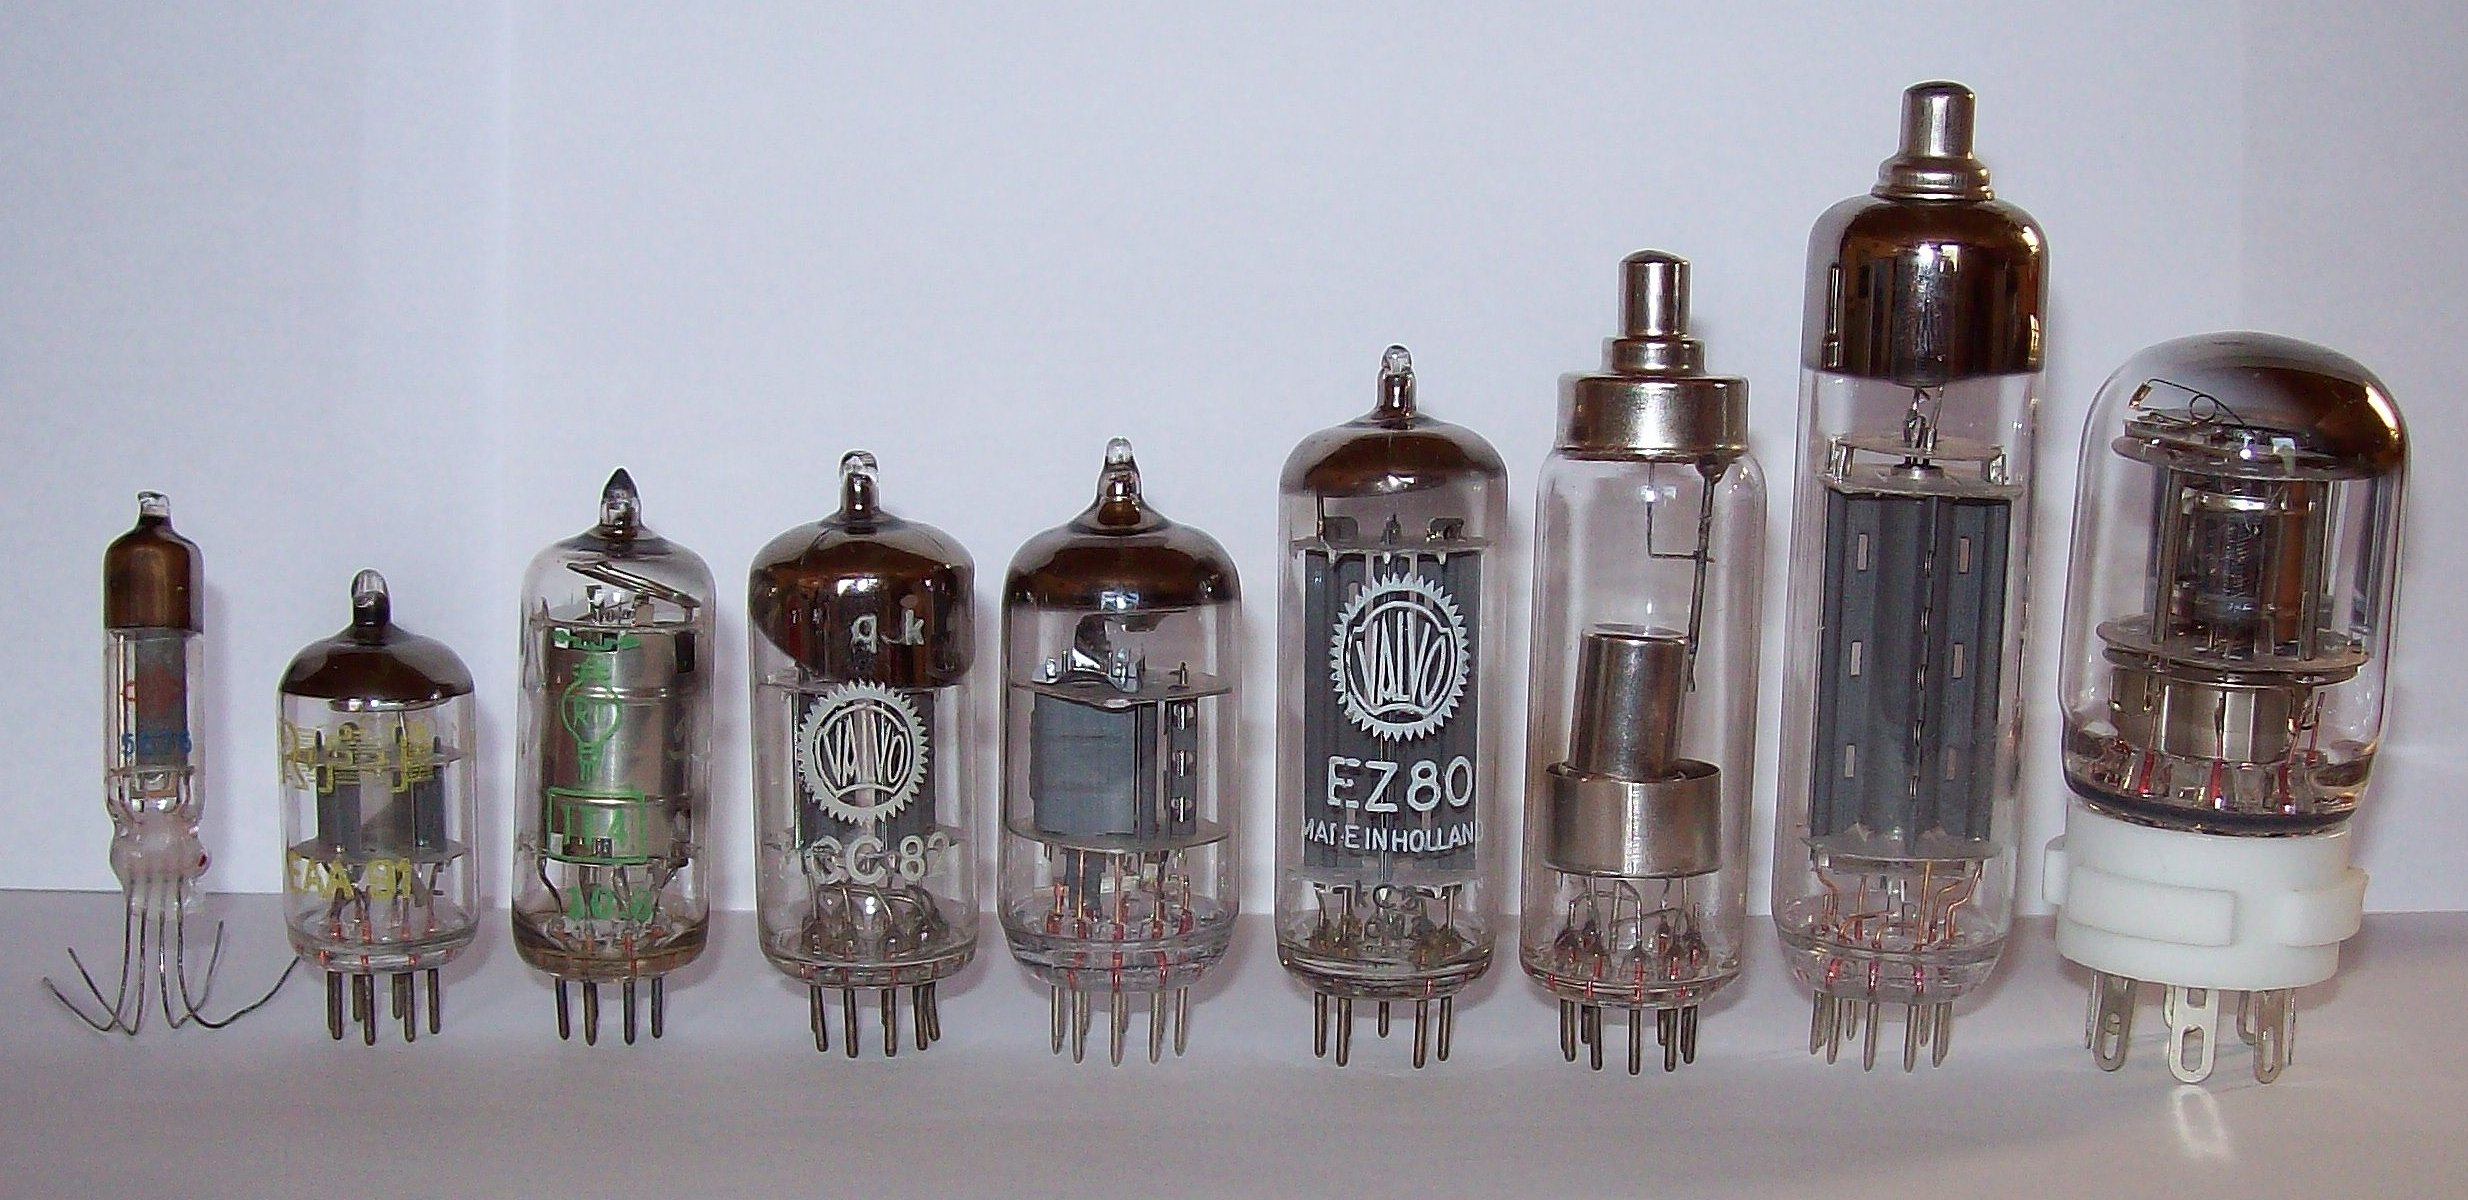
\includegraphics[width=0.7\columnwidth]{chapter01/figure/VacuumTube.jpg}
		\centering
	\caption{Bóng đèn chân không. Nguồn hình ảnh từ Internet.}
	\label{fig:vacuumTube}
\end{figure}

Máy tính ENIAC được lập trình bằng cách thay đổi các công tắc, quá trình này rất phức tạp và nhàm chán. Quá trình lập trình sẽ hiệu quả hơn nếu như các chương trình có thể được biểu diễn dưới dạng phù hợp cho việc lưu trữ nó trong bộ nhớ. Một máy tính sẽ đọc các \emph{lệnh} (instructions) từ bộ nhớ và thực thi chúng. Các chương trình sẽ được cài đặt hoặc thay đổi bằng cách thay đổi một phần bộ nhớ. Ý tưởng này được gọi là \emph{mô hình lưu trữ chương trình} (\emph{stored-program concept}) được phát triển bởi John von Neumann năm 1945 và được dùng cho đến ngày nay. Hiện tại, hầu hết các máy tính đều sử dụng mô hình lưu trữ chương trình hay còn được gọi là mô hình \textbf{von Neumann}.

\begin{figure}[h]
	\centering
		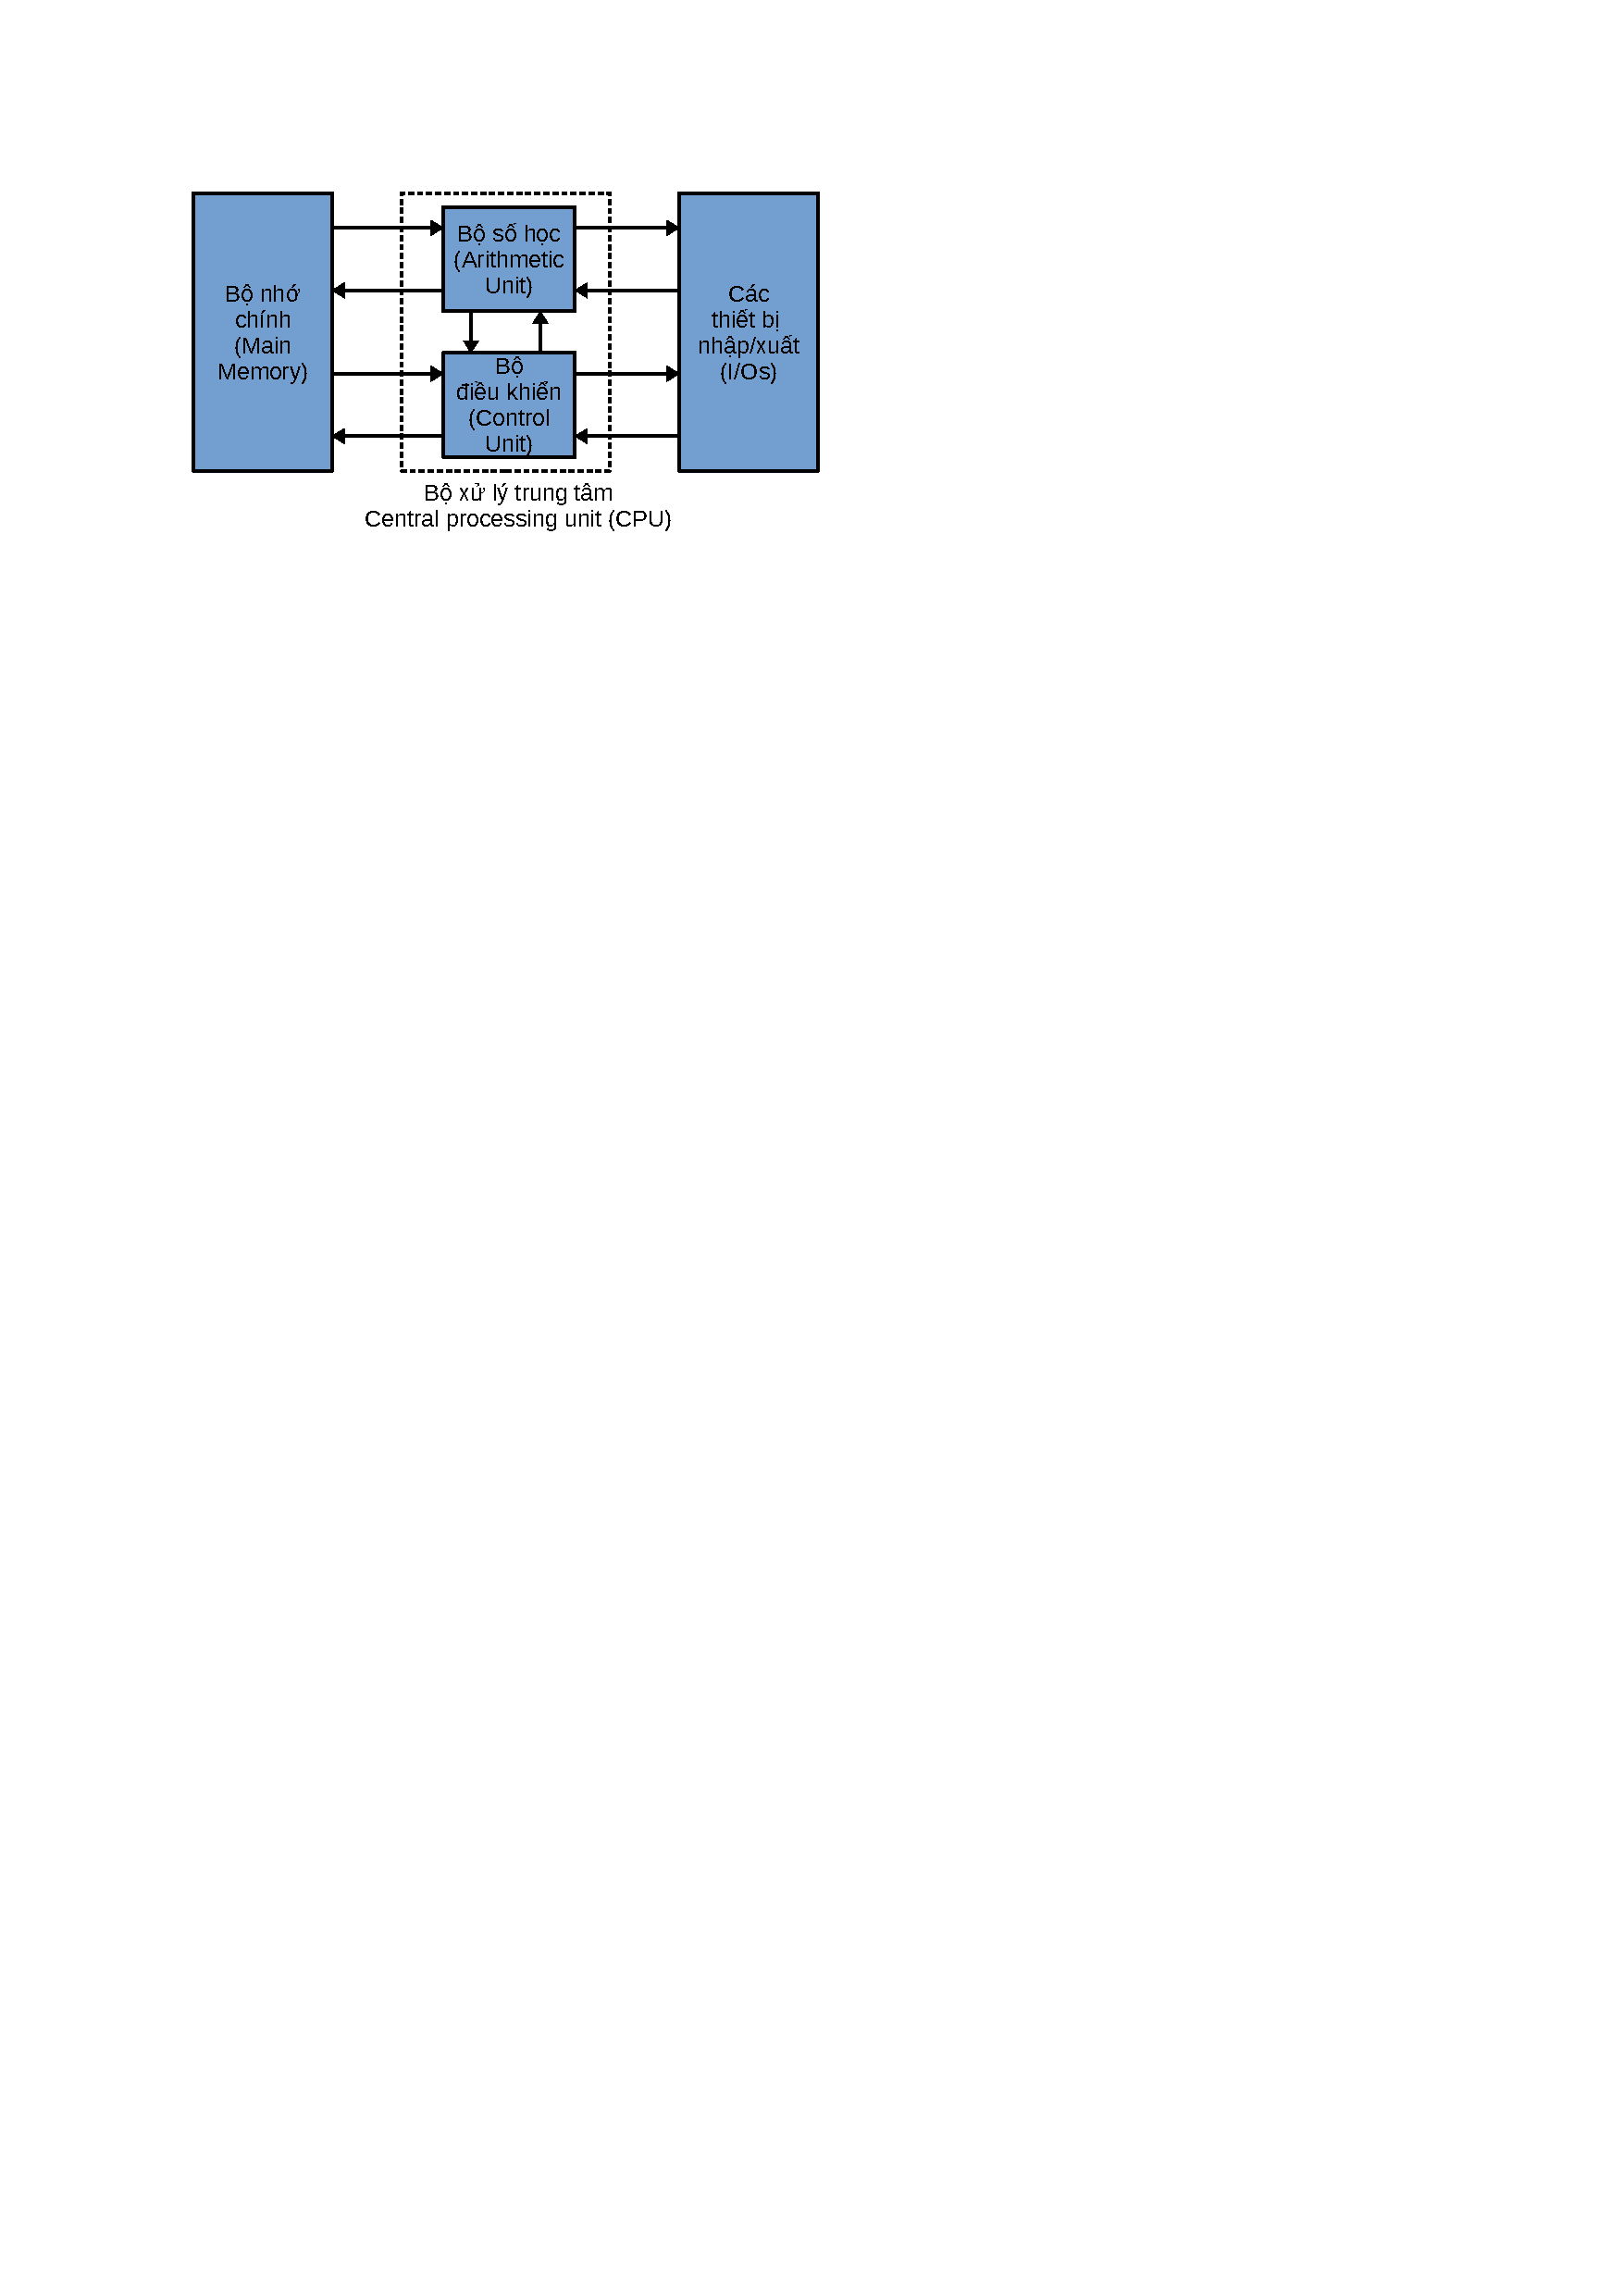
\includegraphics[width=0.7\columnwidth]{chapter01/figure/vonNeumann.pdf}
		\centering
	\caption{Mô hình máy tính von Neumann.}
	\label{fig:vonNeumann}
\end{figure}

Hình~\ref{fig:vonNeumann} trình bày sơ đồ tổng quát của mô hình máy tính von Neumann. Theo mô hình này, một máy tính sẽ có ba thành phần chính là:
\begin{itemize}
	\item \textbf{Bộ nhớ chính} (main memory): là nơi lưu trữ các lệnh của các chương trình và dữ liệu;
	\item \textbf{Bộ xử lý trung tâm} (Central processing unit - CPU): bao gồm hai thành phần là \textbf{Bộ xử lý số học} (Arithmetic unit) có nhiệm vụ tính toán trên dữ liệu nhị phân và \textbf{Bộ điều khiển} (Control unit) có nhiệm vụ diễn giải các lệnh đọc được từ bộ nhớ và thực thi chúng; và
	\item \textbf{Các thiết bị nhập xuất} (Inputs/Outputs): dùng để nhận dữ liệu từ người sử dụng hoặc xuất kết quả cho người sử dụng dưới sự điều khiển của Bộ điều khiển.
\end{itemize}

Năm 1946, John von Neumann và các cộng sự tại Viện Nghiên cứu Nâng cao tại Princeton, Hoa Kỳ bắt đầu thiết kế máy tính IAS dựa trên mô hình lưu trữ chương trình này. Mặc dù phải đến năm 1951, máy tính IAS mới được hoàn thành nhưng nó được xem như là một bản mẫu (prototype) cho tất cả các máy tính đa dụng thế hệ sau. Máy tính IAS có bộ nhớ gồm 1000 vị trí lưu trữ, còn được gọi là \emph{từ nhớ}~\footnote{Không có một định nghĩa chính xác cho thuật ngữ \emph{từ nhớ}. Tổng quát, một từ nhớ là tập hợp có thứ tự các bit và là đơn vị để lưu trữ, truyền đạt và xử lý thông tin trong một máy tính cụ thể. Thông thường một từ nhớ sẽ có kích thước bằng với kích thước lệnh trong các bộ xử lý có kích thước lệnh cố định.} (word) có kích thước 40 bit mỗi từ nhớ dùng để lưu trữ lệnh của các chương trình và dữ liệu. Khác với máy tính ENIAC, máy tính IAS xử lý dữ liệu kiểu nhị phân.

Trong thế hệ máy tính thứ nhất này, hai dòng máy tính được thương mại hóa là UNIVAC (Universal Automatic Computer) và IBM. UNIVAC trong giai đoạn này đã cho ra đời các dòng máy tính UNIVAC I, UNIVAC II, và loạt máy UNIVAC 1100. IBM giới thiệu hai máy tính 701 dùng cho mục đích tính toán khoa học vào năm 1953 và máy tính 702 dùng cho mục đích tính toán các ứng dụng thương mại vào năm 1955. Đây là hai máy tính đầu tiên của dòng máy IBM 700 đã làm nên tên tuổi của IBM trong lĩnh vực sản xuất máy tính.

\subsubsection{Máy tính thế hệ thứ hai}

Sự thay đổi lớn đầu tiên trong các máy tính điện tử đa dụng là sự thay thế các bóng đèn chân không bằng các \textbf{bóng bán dẫn} (transistor). So với các bóng đèn chân không thì các bóng bán dẫn có kích thước nhỏ hơn, giá thành rẻ hơn và sản sinh ra ít nhiệt lượng khi hoạt động hơn. Mặc dù được phát triển lần đầu tiên vào năm 1947 bởi phòng thí nghiệm Bell Labs (Hình~\ref{fig:transistor}), nhưng mãi đến cuối những năm 1950 thì máy tính điện tử đa dụng chế tạo hoàn toàn bằng các bóng bán dẫn mới được thương mại hóa. Năm 1957 được xem là năm kết thúc của máy tính thế hệ thứ nhất để chuyển sang máy tính thế hệ thứ hai, máy tính được chế tạo bằng các bóng bán dẫn. Việc sử dụng các bóng bán dẫn để chế tạo máy tính đánh dấu sự bắt đầu của thế hệ máy tính thứ hai vào năm 1958. Những máy tính đầu tiên trong thế hệ này chứa khoảng 10.000 bóng bán dẫn và tăng dần đến hàng trăm ngàn bóng bán dẫn ở các máy tính ra đời sau trong cùng thế hệ.

\begin{figure}[h]
	\centering
		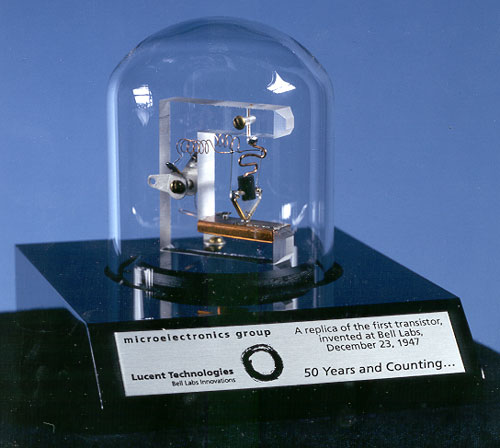
\includegraphics[width=0.7\columnwidth]{chapter01/figure/transistor.jpg}
		\centering
	\caption{Một phiên bản của bóng bán dẫn đầu tiên trên thế giới được phát triển bởi Bell Labs năm 1957.}
	\label{fig:transistor}
\end{figure}

Hai nhà sản xuất đi tiên phong trong việc giới thiệu và ứng dụng công nghệ mới ở giai đoạn này là NCR và RCA. Không lâu sau đó, IBM giới thiệu dòng máy tính 7000. So với dòng máy tính 700 ở thế hệ thứ nhất, các máy tính thuộc dòng 7000 ở thế hệ này của IBM có hiệu suất và dung lượng bộ nhớ tăng đáng kể và kích thước nhỏ hơn nhiều. Kết quả so sánh này cũng đúng khi so sánh giữa các máy được sản xuất trước và sau trong cùng dòng IBM 7000. Điều này được minh họa qua Bảng~\ref{tab:IBM700}, so sánh các máy tính IBM ở hai thế hệ thứ nhất và thứ hai. Ngoài ra, thế hệ máy tính thứ hai còn chứng kiến các sự thay đổi khác như sự xuất hiện của các bộ tính toán số học và luận lý (arithmetic and logic units) cũng như các bộ điều khiển (control units) phức tạp hơn, việc sử dụng các ngôn ngữ lập trình cấp cao, và sự ra đời của phần mềm hệ thống (system software).

\begin{table}[h]
	\small
	\caption{So sánh một số máy tính IBM trong thế hệ thứ nhất và thế hệ thứ hai}
	\label{tab:IBM700}
		\begin{tabular}{l||l|c|l|p{1.7cm}|r}
			\hline
			\textbf{Thế hệ} & \textbf{Tên} & \textbf{Năm sản xuất} & \textbf{Công nghệ} &\textbf{Truy xuất bộ nhớ} & \textbf{Bộ nhớ}\\
			\hline
			\hline
			\multirow{3}{*}{I} & 701 &  1952 & Đèn chân không & 30 $\mu$s& 2-4 K\\
			\cline{2-6}
			& 704 & 1955 & Đèn chân không & 12 $\mu$s & 4-32 K\\
			\cline{2-6}
			& 709 & 1958 & Đèn chân không & 12 $\mu$s & 32 K \\
			\hline
			\hline
			\multirow{3}{*}{II} & 7090 & 1960 & Bóng bán dẫn & 2.18 $\mu$s& 32 K\\
			\cline{2-6}
			& 7094 I & 1962 & Bóng bán dẫn & 2.0 $\mu$s& 32 K\\
			\cline{2-6}
			& 7094 II & 1964 & Bóng bán dẫn & 1.4 $\mu$s& 32 K\\
			\hline
		\end{tabular}
\end{table}

\subsubsection{Máy tính thế hệ thứ ba}
Mặc dù các bóng bán dẫn được sử dụng thay thế các bóng đèn chân không trong sản xuất máy tính và đạt được những cải tiến, tuy vậy các bóng bản dẫn này được chế tạo và đóng gói riêng biệt. Một máy tính hay đơn giản hơn là một thiết bị điện tử sẽ được chế tạo bằng cách nối dây kết nối những bóng bán dẫn này lại với nhau trên một bảng mạch. Quá trình chế tạo máy tính từ bóng bán dẫn cho tới các bảng mạch tốn kém và phức tạp đặc biệt là khi nhu cầu tính toán ngày càng cao. Khi số lượng bóng bán dẫn cần thiết cho một máy tính ngày càng lớn thì các máy tính chế tạo theo công nghệ hiện tại không đáp ứng được; do đó thế hệ máy tính thứ ba dựa trên mạch tích hợp (integrated circuits) ra đời.

Mạch tích hợp được định nghĩa là: \emph{``một thiết bị được tạo thành từ các thành phần điện tử như là các bóng bán dẫn hay các điện trở kết nối với nhau được hiện thực trên một mảnh nhỏ vật liệu bán dẫn (semiconducting material)''}. Mạch tích hợp đầu tiên hoạt động được trên thế giới được giới thiệu vào tháng 9 năm 1958 chỉ gồm một vài bóng bán dẫn và có kích thước phần mạch chính là 11.11 mm$\times$1.59 mm như Hình~\ref{fig:IC}. Sự ra đời của mạch tích hợp cũng là sự bắt đầu của máy tính thế hệ thứ ba, máy tính chế tạo bằng các mạch tích hợp.

\begin{figure}[h]
	\centering
		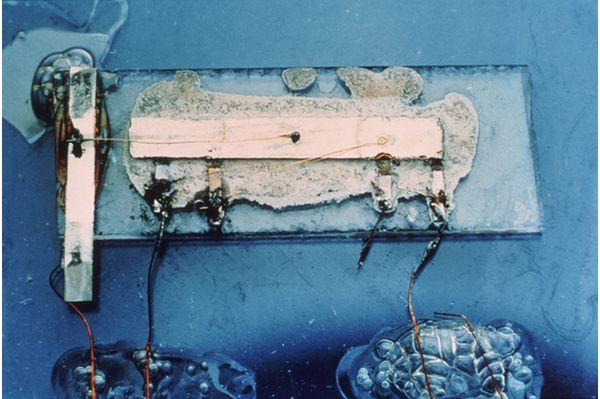
\includegraphics[width=0.7\columnwidth]{chapter01/figure/IC.jpg}
		\centering
	\caption{Mạch tích hợp hoạt động được đầu tiên trên thế giới.}
	\label{fig:IC}
\end{figure}

Các mạch tích hợp ở giai đoạn đầu chỉ bao gồm một số lượng rất nhỏ bán dẫn trên một chip. Trải qua quá trình phát triển liên tục, đến năm 2014 đã có thể tích hợp trên 20 tỉ bóng bán dẫn trên một chip. Tháng 7 năm 2016, Altera (một hãng công nghệ sản xuất chip tái cấu hình của Mỹ đã được mua lại bởi tập đoàn Intel) đã công bố chip được tích hợp trên 30 tỉ bóng bán dẫn. Sự phát triển của số lượng bóng bán dẫn trên một chip trong giai đoạn vừa qua tuân theo tiên đoán của Gordon Moore (còn được gọi là định luận Moore), một nhà đồng sáng lập Intel vào những năm 1970 đó là số lượng bóng bán dẫn trên một chip sẽ tăng gấp đôi sau mỗi 18 đến 24 tháng. Hình~\ref{fig:Transistor_Count} thống kê số lượng các bóng bán dẫn trên các bộ xử lý nổi tiếng từ năm 1971 đến năm 2011 và so sánh với định luật Moore (đường thẳng). Có thể thấy rằng, sự phát triển về số lượng bóng bán dẫn của các mạch tích hợp nói chung và các bộ xử lý nói riêng tuân theo tiên đoán của Moore phát biểu vào những năm 1970.

%\begin{figure}[h]
\begin{sidewaysfigure}
	\centering
		%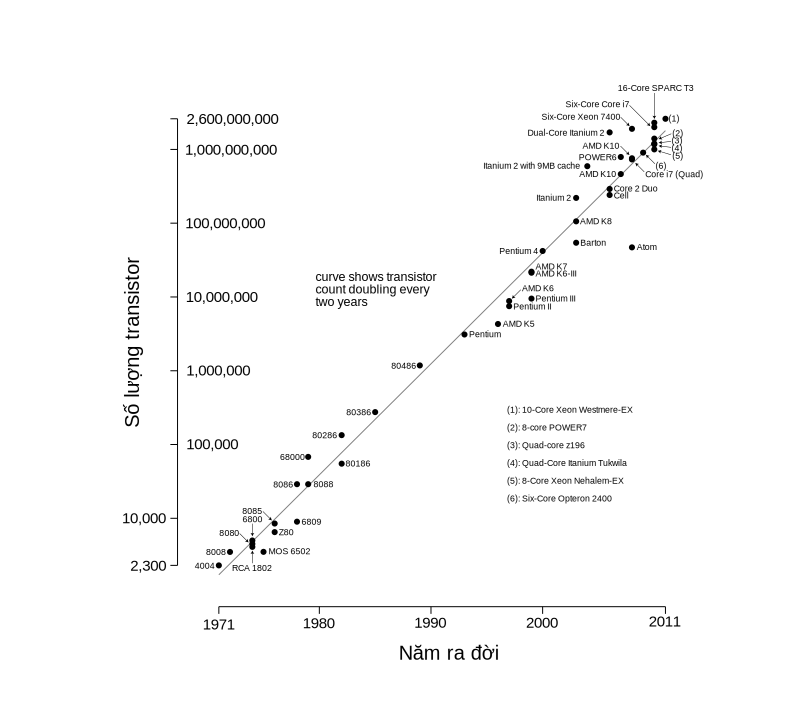
\includegraphics[width=1.0\columnwidth]{chapter01/figure/Transistor_Count_pdf}
		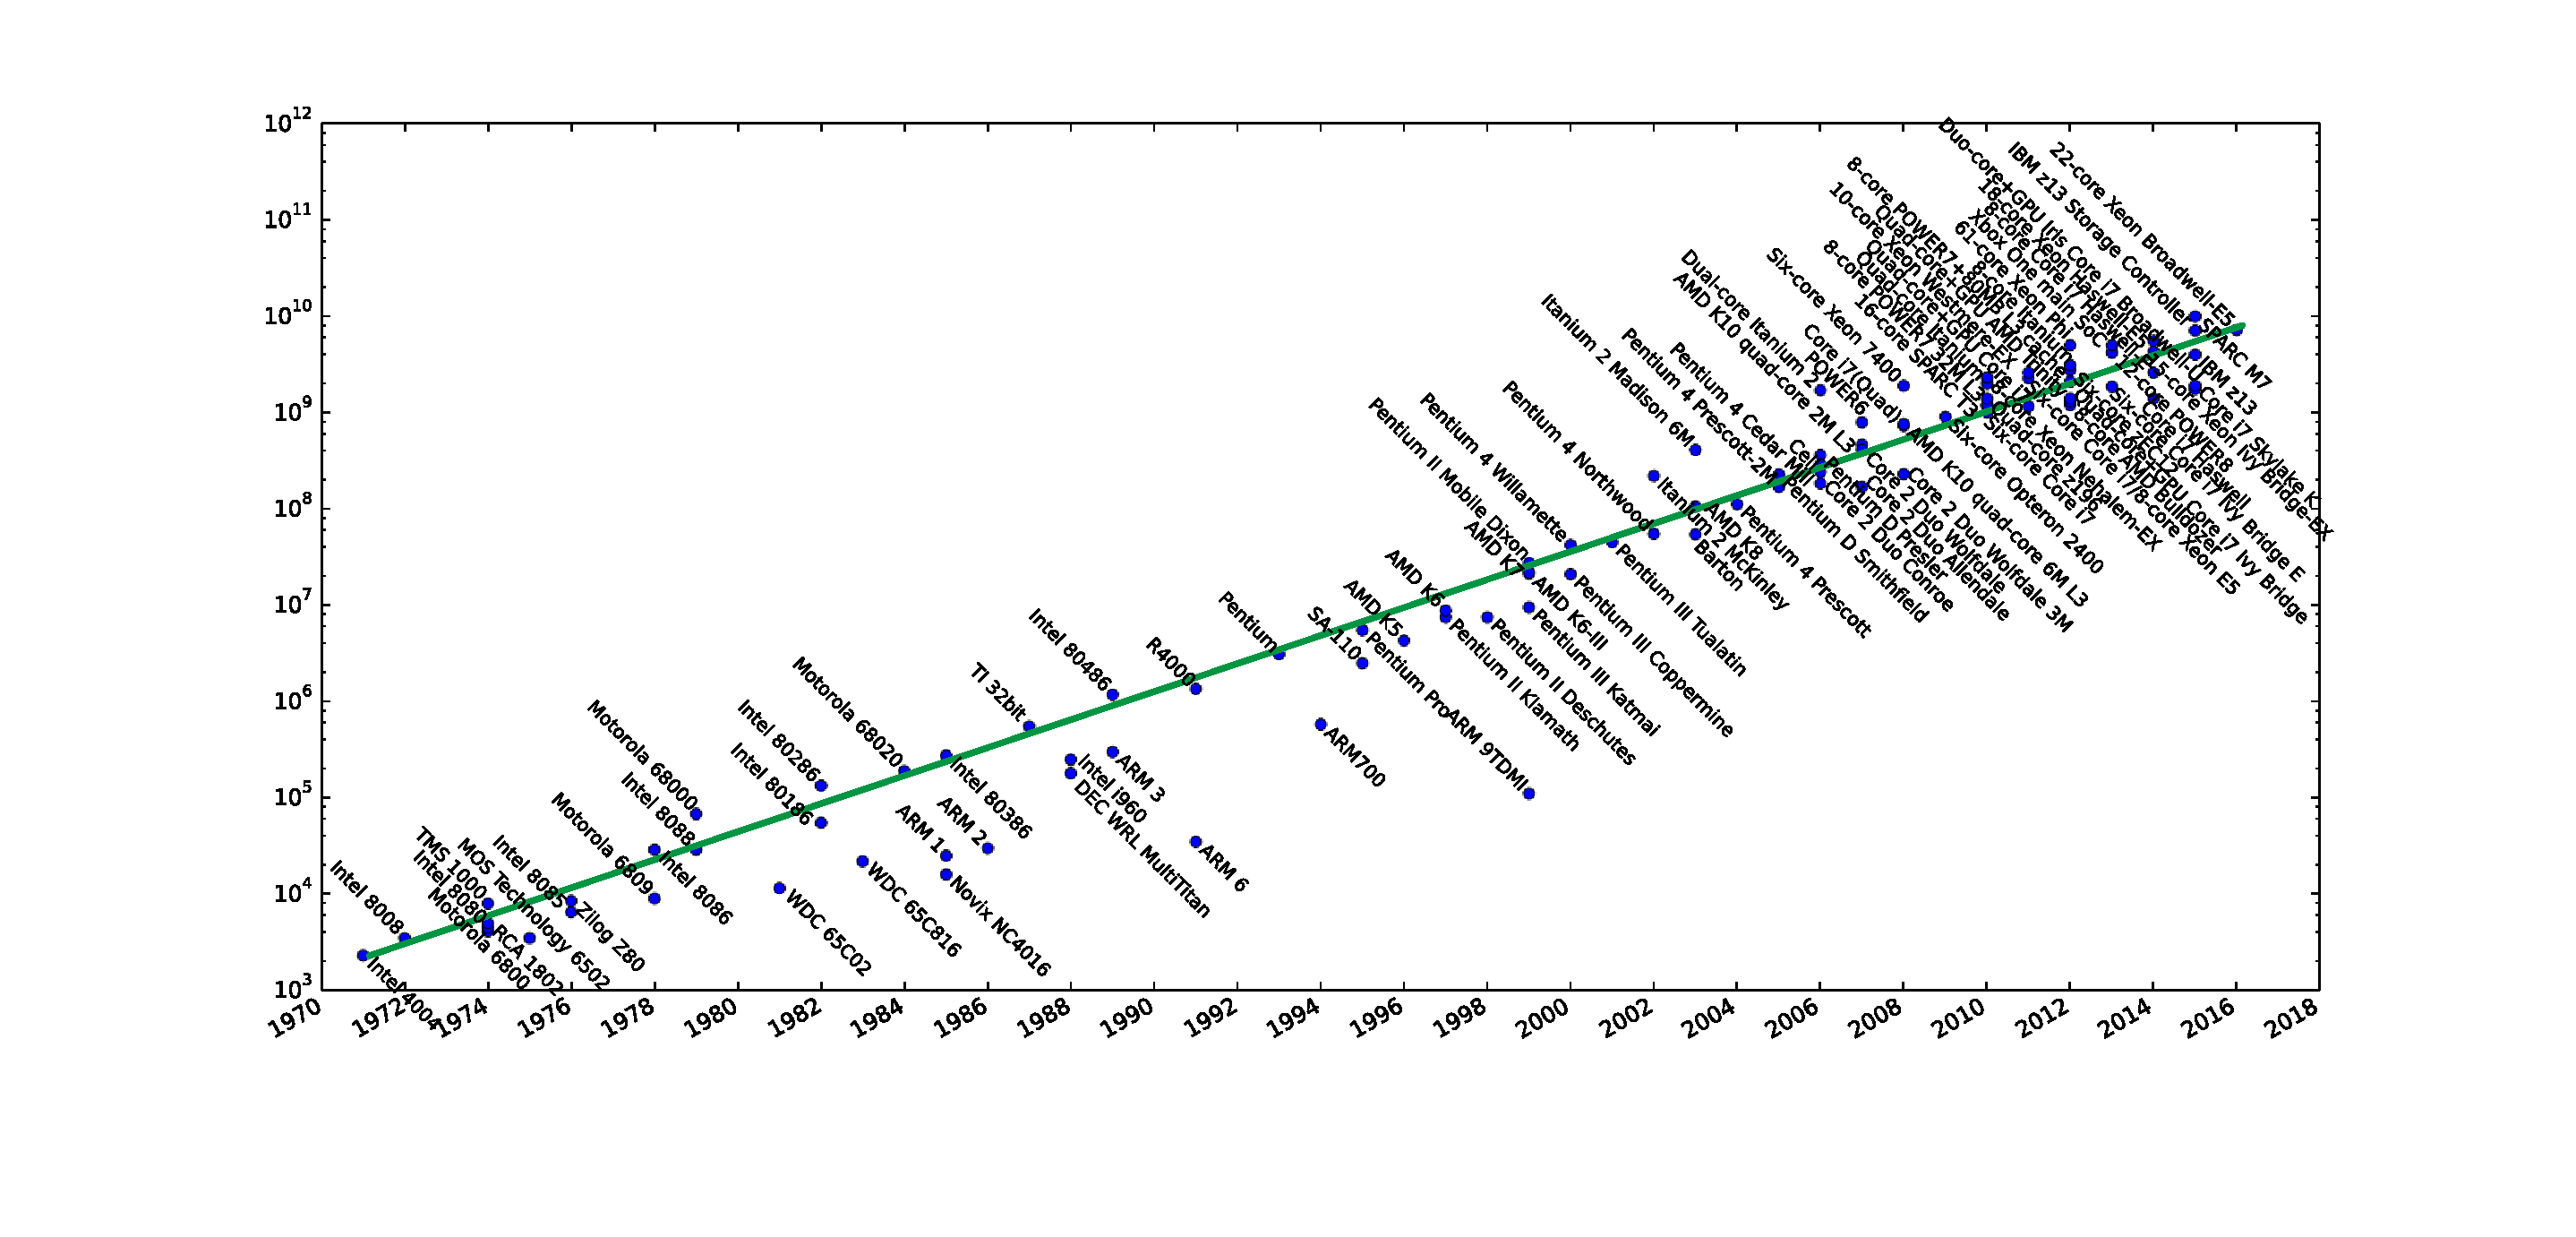
\includegraphics[width=1.0\columnwidth]{chapter01/figure/transistors}
		\centering
	\caption{So sánh số lượng bóng bán dẫn trên các bộ xử lý và định luật Moore. Nguồn số liệu \url{https://en.wikipedia.org/wiki/Transistor_count}}
	\label{fig:Transistor_Count}
%\end{figure}
\end{sidewaysfigure}

Hai dòng máy tính nổi tiếng trong thế hệ này là: IBM System/360 và DEC PDP-8. Dòng máy tính IBM System/360 ra đời năm 1964 đánh dấu sự thành công của IBM trong lĩnh vực sản xuất máy tính ở giai đoạn này khi chiếm đến 70\% thị trường máy tính trên toàn thế giới. Tuy nhiên do chuyển hoàn toàn sang công nghệ mạch tích hợp mới nên các máy tính IBM System/360 không tương thích với dòng máy tính trước đó của IBM. Dòng máy tính IBM System/360 này bao gồm nhiều mẫu khác nhau phục vụ cho nhu cầu khác nhau của khách hàng về khả năng tính toán và giá thành. Tuy nhiên, các máy tính trong dòng máy tính IBM System/360 này sử dụng cùng một tập lệnh và cùng một hệ điều hành; do đó khi người sử dụng nâng cấp máy tính thì không cần phải thay đổi chương trình đang sử dụng. Dòng máy này không những là kim chỉ nam cho các dòng máy tính thế hệ sau của IBM mà còn có ảnh hưởng rất lớn đến cả ngành công nghiệp máy tính.

Đến thời điểm bắt đầu của thế hệ máy tính thứ ba, hầu hết các máy tính có hiệu suất trung bình trở lên đều đòi hỏi phải được đặt trong một phòng máy lạnh và có giá thành lên đến hàng trăm ngàn USD. Cùng năm với sự ra đời của dòng máy tính IBM System/360, hãng DEC (Digital Equipment Corporation) giới thiệu máy tính nhỏ PDP-8 dùng công nghệ mạch tích hợp đủ nhỏ để có thể đặt trên bàn ở các phòng thí nghiệm. Mặc dù máy tính PDP-8 không có đầy đủ các chức năng như một máy tính cỡ lớn như IBM System/360, nhưng với giá thành khá rẻ so với các dòng máy cỡ lớn chỉ khoảng 16.000 USD thì máy tính PDP-8 thu hút được lượng khá lớn người sử dụng.

\subsubsection{Máy tính thế hệ thứ tư}

Sau thế hệ thứ ba, các nhà khoa học vẫn chưa thống nhất với nhau về định nghĩa các thế hệ máy tính tiếp theo. Mặc dù cho đến hiện nay, công nghệ mạch tích hợp dùng các bóng bán dẫn vẫn đang được sử dụng rộng rãi, tuy nhiên số lượng bóng bán dẫn được tích hợp trên một chip đã tăng rất đáng kể và tuân theo định luật Moore. Các mạch tích hợp được chia thành các loại như trong Bảng~\ref{tab:VLSI} dựa vào số lượng bóng bán dẫn được tích hợp trên một chip. Dựa trên sự phân loại các mạch tích hợp, một số nhà nghiên cứu đề nghị chia các máy tính sau thế hệ thứ ba thành các thế hệ máy tính LSI, VLSI và ULSI. Tuy nhiên, do công nghệ chế tạo và kiến trúc của các máy tính này là gần như tương đồng, nên thường được gọi chung là máy tính thế hệ thứ tư. Đặc điểm của máy tính thế hệ thứ tư này là sử dụng bộ nhớ bán dẫn và các vi xử lý (microprocessor).

Ban đầu khi mạch tích hợp ra đời, mạch tích hợp chủ yếu được dùng để chế tạo các bộ xử lý. Bộ nhớ của các máy tính ra đời trong những năm 1950 và 1960 dùng vật liệu sắt từ (ferromagnetic material). Hai vấn đề lớn nhất của bộ nhớ dùng vật liệu sắt từ là giá thành và dữ liệu bị xóa sau khi đọc. Năm 1970, hãng công nghệ Fairchild giới thiệu \textbf{bộ nhớ bán dẫn} (semiconductor memory) đầu tiên trên thế giới giải quyết được vấn đề xóa dữ liệu khi đọc và có tốc độ đọc cao hơn hẳn bộ nhớ dùng vật liệu sắt từ. Đến năm 1974, khi giá thành sản xuất bộ nhớ bán dẫn được giảm xuống, bộ nhớ bán dẫn được dùng trong hầu hết các máy tính.

\begin{table}[!h]
	\small
	\caption{Các loại mạch tích hợp}
	\label{tab:VLSI}
		\begin{tabular}{l||c|r|r}
			\hline
			\textbf{Tên} & \textbf{Năm ra đời} & \textbf{Số lượng bóng bán dẫn} & \textbf{Số lượng cổng luận lý} \\
			\hline
			\hline
			SSI & 1964 & 1 đến 10 & 1 đến 12 \\
			\hline
			MSI & 1968 & 10 đến 500 & 13 đến 99 \\
			\hline
			LSI & 1971 & 500 đến 20.000 & 100 đến 9.999 \\
			\hline
			VLSI & 1980 & 20.000 đến 1.000.000 & 10.000 đến 99.999 \\
			\hline
			ULSI & 1984 & 1.000.000 trở lên & 100.000 trở lên\\
			\hline
		\end{tabular}
\end{table}

Đi đôi với sự ra đời bộ nhớ bán dẫn, công nghệ sản xuất bộ xử lý cũng có những bước phát triển vượt bậc. Ngày càng nhiều bộ phận thành phần được tích hợp trên cùng một chip, do đó số lượng chip cần dùng để xây dựng nên một bộ xử lý càng ít. Năm 1971 chứng kiến một sự thay đổi toàn diện trong lĩnh vực chế tạo bộ xử lý máy tính đó là sự ra đời của bộ \textbf{vi xử lý} (microprocessor) 4004 của Intel. Chip Intel 4004 là một chip đơn đầu tiên chứa tất cả các bộ phận thành phần của một bộ xử lý trung tâm của máy tính. Mặc dù chỉ có thể thực hiện được phép cộng hai số 4 bit và thực hiện phép nhân bằng cách cộng nhiều lần nhưng bộ vi xử lý 4004 đánh dấu quá trình phát triển mạnh mẽ của các bộ vi xử lý cả về khả năng tính toán lẫn công suất tiêu thụ.

Năm 1972 Intel giới thiệu bộ vi xử lý thế hệ tiếp theo của 4004 là 8008 có khả năng xử lý 8 bit thay vì 4 bit như 4004. Tuy nhiên cả hai bộ vi xử lý 4004 và 8008 đều chỉ được sử dụng cho các ứng dụng chuyên biệt. Năm 1974 chứng kiến sự ra đời của vi xử lý đa dụng (general-purpose microprocessor) 8 bit đầu tiên Intel 8080. Đây là mốc đánh dấu cho thế hệ máy tính thứ 4, thế hệ máy tính dùng các bộ vi xử lý và bộ nhớ bán dẫn. Trong những năm tiếp theo sau, các hãng công nghệ liên tục giới thiệu các bộ xử lý các thế hệ tiếp có khả năng xử lý 16, 32, và 64 bit sử dụng các công nghệ chế tạo mạch tích hợp tiên tiến có kích thước các bóng bán dẫn ngày càng nhỏ. Bảng~\ref{tab:Intel} so sánh các bộ xử lý tiêu biểu của Intel trong giai đoạn những năm 1970 và giai đoạn gần đây.

\begin{table}[htb]
	\small
	\caption{Sự phát triển của các bộ xử lý Intel}
	\label{tab:Intel}
	\caption*{Giai đoạn những năm 1970}
		\begin{tabular}{l||c|c|c|c|c}
			\hline
			& \textbf{4004} & \textbf{8008} & \textbf{8080} & \textbf{8086} & \textbf{8088}\\
			\hline
			\hline
			Năm sản xuất & 1971 & 1972 & 1974 & 1978 & 1979 \\
			\hline
			Tần số clock & 108 kHz  & 108 kHz & 2 MHz & $5\to10$ MHz & $5\to8$ MHz \\
			\hline
			Độ rộng bus & 4 bit& 8 bit& 8 bit& 16 bit& 8 bit\\
			\hline
			Số lượng BBD$^{1}$ & 2.300 & 3.500 & 6.000 & 29.000 & 29.000 \\
			\hline
			Kích thước BBD & 10 ${\mu}m$ & & 6 mm & 3 mm & 6 mm\\
			\hline
			Quản lý bộ nhớ & 640 Bytes & 16 KB & 64 KB & 1 MB & 1 MB\\
			\hline
		\end{tabular}
		\begin{itemize} [] \footnotesize \itemsep1pt \parskip0pt \parsep0pt
        \item $^{(1)}$BDD: bóng bán dẫn (transistor)
		\end{itemize}
		\caption*{Giai đoạn gần đây}
				\begin{tabular}{l||c|c|c|c}
			\hline
			 & \textbf{Pentium 4} & \textbf{Core 2 Duo} & \textbf{Core i7-920} & \textbf{Core i7-6700K} \\
			\hline
				\hline
			Năm sản xuất & 2000 & 2006 & 2008 & 8/2015 \\
			\hline
			Tần số clock & 1.3-1.8 GHz  & 1.06-1.12 GHz & 2.66 GHz & 4 GHz  \\
			\hline
			Độ rộng bus & 64 bit & 64 bit & 64 bit & 64 bit\\
			\hline
			Số lượng BBD$^{1}$ & 42 triệu & 167 triệu & 731 triệu & 1.35 tỉ  \\
			\hline
			Kích thước BBD & 180 nm & 65 nm & 45 nm & 14 nm \\
			\hline
			Quản lý bộ nhớ & 64 GB & 64 GB & 24 GB & 64 GB \\
			\hline
			Bộ đệm & 256 KB L2 & 2 MB L2 & 6 MB L2 & 8 MB L2 \\ 
			\hline
		\end{tabular}
\end{table}

\subsection{Phân loại máy tính}
Mặc dù các máy tính hiện nay được sản xuất dưới cùng một công nghệ chế tạo phần cứng cho cả bộ vi xử lý và bộ nhớ cũng như đều dựa trên mô hình máy tính von Neumann, các máy tính được dùng trong những nhóm ứng dụng khác nhau sẽ có những đặc điểm và yêu cầu khác nhau. Một cách tổng quát, các máy tính có thể được phân chia thành bốn loại khác nhau.

\subsubsection{Máy tính cá nhân}
Máy tính cá nhân (Personal Computer - PC) là loại máy tính có thể nói là phổ biến nhất hiện nay. Khái niệm máy tính cá nhân ra đời trong khoảng 35 năm trở lại đây. Các máy tính cá nhân có những đặc điểm riêng biệt là hiệu suất tốt cho một người sử dụng tại một thời điểm, giá thành thấp và thường thực hiện những ứng dụng của bên thứ ba (third-party software).

\subsubsection{Máy chủ}
Máy chủ (Server) là khái niệm để chỉ những máy tính thường được truy xuất chỉ thông qua mạng (network). Các máy chủ thường được dùng để thực hiện một ứng dụng phức tạp - ví dụ các ứng dụng tính toán khoa học - hoặc thực thi nhiều ứng dụng nhỏ - ví dụ các ứng dụng cấu thành một trang mạng (website). Các máy chủ thường được xây dựng từ những công nghệ và thành phần cơ bản giống với máy tính cá nhân nhưng cung cấp khả năng tính toán mạnh hơn, khả năng lưu trữ và truy xuất thiết bị ngoại vi lớn hơn. Máy chủ hiện nay bao gồm rất nhiều loại có giá thành và sức mạnh khác nhau. Máy chủ dòng thấp nhất có thể chỉ là một máy tính cá nhân và có giá trong khoảng một ngàn USD. Các máy chủ dòng thấp này thông thường chỉ được dùng để lưu trữ dữ liệu hoặc thực thi những ứng dụng nhỏ hoặc những trang mạng đơn giản. Bên cạnh đó, có những máy chủ có sức mạnh tính toán rất lớn và giá thành rất cao để phục vụ cho nhiều ứng dụng phức tạp và nhiều người dùng cùng lúc. Yêu cầu quan trọng nhất của các máy chủ là độ tin cậy cao (reliability) bởi vì mọi sự hư hỏng trên các máy chủ sẽ có ảnh hưởng đến rất nhiều người.

\subsubsection{Siêu máy tính}
Khái niệm siêu máy tính (Supercomputer) để chỉ những máy tính có khả năng tính toán vô cùng lớn. Các siêu máy tính này thường có đến hàng chục ngàn bộ xử lý, dung lượng lưu trữ lên đến nhiều terabytes\footnote{1 terabyte bằng $2^{40}$ byte.} và có giá thành lên đến hàng trăm triệu USD. Các siêu máy tính này dùng để tính toán những ứng dụng khoa học đòi hỏi sức mạnh tính toán rất lớn như dự báo thời tiết, tìm kiếm mỏ dầu, các bài toán so trùng chuỗi DNA,... Danh sách các siêu máy tính mạnh nhất thế giới có thể tìm thấy tại trang mạng \url{www.top500.org}. Mặc dù đây là loại máy tính có sức mạnh tính toán lớn nhất thế giới nhưng số lượng của nó trên thị trường là ít nhất so với ba loại còn lại.

\subsubsection{Máy tính nhúng}
Máy tính nhúng (Embedded computer) là loại máy tính có số lượng cũng như các mức độ hiệu suất khác nhau nhiều nhất hiện nay. Máy tính nhúng bao gồm từ các bộ vi xử lý có thể tìm thấy trong xe hơi, máy tính trong các thiết bị truyền hình thông minh, cho đến mạng các bộ xử lý (network of processors) dùng điều khiển các chuyến bay. Máy tính nhúng được thiết kế để có thể thực thi hiệu quả nhất chỉ một ứng dụng hoặc một tập ứng dụng liên quan nhau. Máy tính nhúng thường được đóng gói cùng với các thiết bị phần cứng khác thành một hệ thống duy nhất. Điều đặc biệt là hầu hết người sử dụng thường không nhận thấy rằng mình đang sử dụng một máy tính. Sự bùng nổ của các máy tính nhúng đặc biệt là trong các thiết bị điện tử cầm tay làm xuất hiện \emph{kỷ nguyên hậu máy tính cá nhân} (PostPC-era) khi mà số lượng máy tính cá nhân (PC) bán ra hàng năm ít hơn nhiều so với các loại máy tính điện tử cầm tay khác.

\subsection{Kỷ nguyên hậu máy tính cá nhân}
Hình~\ref{fig:PostPC_chart} so sánh số lượng các điện thoại thông minh (smartphones) và các máy tính bảng (tablets) bán ra so với số lượng máy tính cá nhân truyền thống (PCs) từ năm 2010 đến nay và dự báo đến năm 2020. Có thể thấy rằng, hiện tại và trong tương lai gần, các máy tính cá nhân truyền thống đang bão hòa về số lượng bán ra trong khi số lượng máy tính bảng và số lượng điện thoại thông minh gia tăng không ngừng.

\begin{figure}[!h]
	\centering
		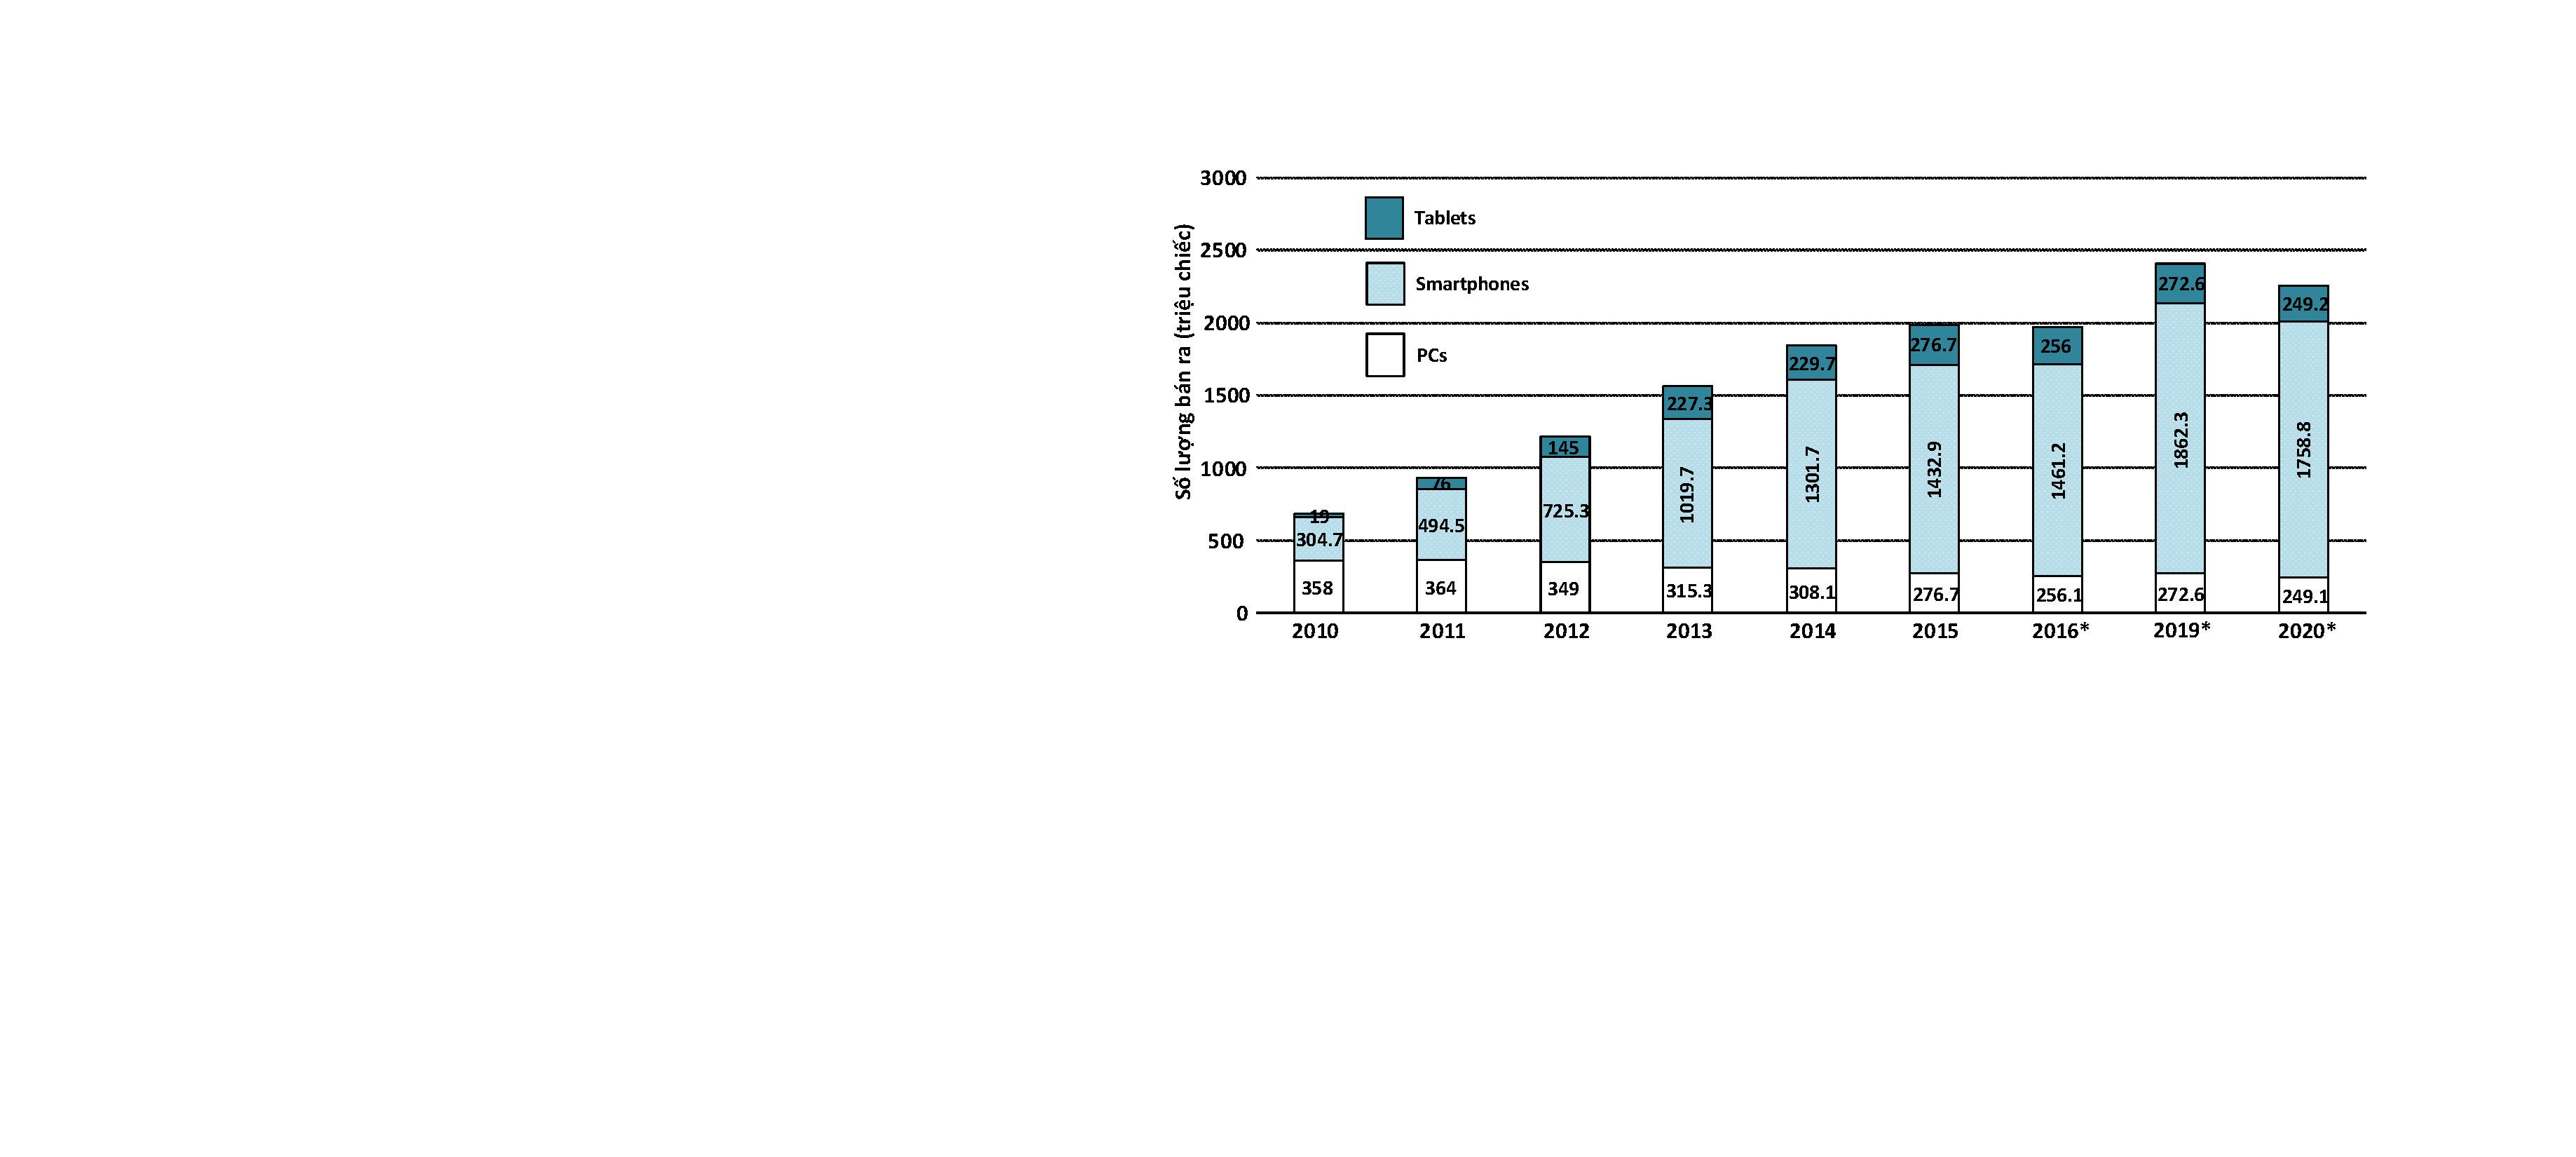
\includegraphics[width=0.95\columnwidth]{chapter01/figure/PostPC_chart.pdf}
		\centering
	\caption{Số lượng các máy tính, máy tính bảng và điện thoại thông minh bán ra. Nguồn dữ liệu \url{https://www.statista.com}.}
	\label{fig:PostPC_chart}
\end{figure}

Các máy tính cá nhân đang dần dần được thay thế bằng các thiết bị cá nhân di động (personal mobile device - PMD). Các thiết bị cá nhân di động này thường là các thiết bị nhỏ có kết nối không dây có thể truy cập vào mạng internet với giá thành vài trăm USD. Các thiết bị cá nhân này hoạt động bằng pin và các phần mềm ứng dụng (thường được gọi là ``apps'') có thể được tải về và cài đặt. Khác với các máy tính cá nhân, các thiết bị cá nhân di động thường không có bàn phím và chuột mà thay thế bằng các màn hình cảm ứng hoặc thậm chí là được điều khiển bằng giọng nói. Ví dụ rõ ràng nhất việc các thiết bị di động cá nhân hiện tại đang thay thế dần các máy tính cá nhân là sự bùng nổ các máy tính bảng và các điện thoại thông minh, và tương lai có thể là các kính điện tử thông minh (smart glass).

\section{Các mức trừu tượng của chương trình máy tính}
Một ứng dụng cơ bản như ứng dụng xử lý văn bản hoặc ứng dụng tính toán bảng tính có thể được phát triển bởi hàng triệu dòng lệnh và sử dụng những thư viện phần mềm phức tạp hiện thực các hàm phức tạp. Trong khi đó, phần cứng máy tính chỉ có thể xử lý những lệnh mức thấp rất đơn giản. Để chuyển đổi từ các ứng dụng phức tạp đến các lệnh phần cứng đơn giản, rất nhiều lớp phần mềm khác nhau tham gia vào việc biên dịch hoặc thông dịch ứng dụng thành các lệnh máy tính đơn giản. Các mức độ hiện thực ứng dụng sử dụng các ngôn ngữ có mức độ phức tạp khác nhau được gọi là các \emph{mức trừu tượng} (abstraction).

\subsection{Ngôn ngữ máy}
Nếu như tiếng Anh sử dụng một bảng chữ cái có 26 ký tự thì bảng chữ cái của máy tính chỉ gồm hai ký tự 0 và 1 tương ứng với hai trạng thái của các mạch điện tử là \emph{đóng} và \emph{ngắt} (\emph{on} và \emph{off}). Mỗi ký tự 0 hoặc 1 được gọi là các ký số nhị phân - \emph{bit} (binary digit); và ngôn ngữ của máy tính (machine language) là ngôn ngữ dựa trên các số nhị phân này. Để điều khiển được máy tính và yêu cầu máy tính thực hiện những công việc cụ thể nào đó, người lập trình phải ``nói'' ngôn ngữ máy tính. Các tác vụ mà người lập trình có thể yêu cầu máy tính làm trực tiếp được gọi là các \emph{lệnh máy}. Lệnh máy là một chuỗi các bit nhị phân mà máy tính có thể hiểu được và thực thi được. Ví dụ một lệnh máy chứa các số nhị phân:\\
\\
\begin{minipage}[l]{8cm}
\leftskip=0.5cm
{\ttfamily 1000110010100000}\\
\end{minipage}
\\
sẽ yêu cầu máy tính thực hiện việc cộng hai số. Chi tiết của các lệnh máy sẽ được giới thiệu trong Chương~\ref{chp:02}. Lệnh máy là lệnh có mức trừu tượng đối với máy tính là thấp nhất vì máy tính có thể hiểu một cách trực tiếp.

\subsection{Hợp ngữ}
Những lập trình viên đầu tiên giao tiếp và điều khiển máy tính thông qua các lệnh máy, là các chuỗi số nhị phân. Tuy nhiên, lập trình cách này rất tốn thời gian và công sức. Do đó, những ký hiệu mới gần với suy nghĩ của con người được phát minh và các ký hiệu này sau đó sẽ được chuyển đổi ra ngôn ngữ máy bằng tay. Tuy nhiên quá trình chuyển đổi này vẫn còn phức tạp và tốn nhiều công sức. Tiếp sau đó, ý tưởng \emph{dùng máy tính để lập trình máy tính} ra đời khi các chương trình được gọi là \textbf{trình hợp dịch} (assembler) được thiết kế để chuyển đổi các lệnh dưới dạng ký hiệu thành các chuỗi nhị phân. Các lệnh được viết dưới dạng ký hiệu được gọi là \emph{hợp ngữ} (assembly language). Ví dụ lệnh hợp ngữ:\\
\begin{minipage}[l]{8cm}
\leftskip=0.5cm
{\ttfamily add A, B}
\end{minipage}\\
sẽ có lệnh máy tương đương với chuỗi nhị phân đã được giới thiệu trong phần trước. Các lệnh hợp ngữ không thể được xử lý trực tiếp bởi phần cứng máy tính mà phải thông qua trình hợp dịch để chuyển đổi thành các lệnh máy. Do đó, mức trừu tượng của hợp ngữ đối với máy tính sẽ cao hơn lệnh máy. Một lệnh hợp ngữ tương đương với duy nhất một lệnh máy.

\subsection{Ngôn ngữ lập trình cấp cao}
Mặc dù hợp ngữ đã cải thiện đáng kể những khó khăn gặp phải khi lập trình với ngôn ngữ máy, nhưng hợp ngữ vẫn khác xa so với những ký hiệu và cách thức một nhà khoa học ở một lĩnh vực nào đó như toán học hay hóa học mong muốn để mô phỏng một vấn đề khoa học hoặc một nhà kế toán dùng để tính toán một vấn đề tài chính. Hợp ngữ vẫn đòi hỏi người lập trình viết từng dòng lệnh mà máy tính sẽ thực hiện theo, điều này làm cho người lập trình cần phải suy nghĩ giống như máy tính.

Ngôn ngữ lập trình cấp cao (high-level programming language) ra đời nhằm giải quyết những khó khăn khi lập trình với hợp ngữ và nâng cao hiệu quả của việc lập trình. Một chương trình sẽ được dùng để chuyển đổi các chương trình viết bằng ngôn ngữ lập trình cấp cao sang hợp ngữ được gọi là \emph{trình biên dịch} (compiler). Sự ra đời của các ngôn ngữ lập trình cấp cao và trình biên dịch là một trong những bước tiến quan trọng trong giai đoạn đầu của ngành công nghiệp điện toán. Đối với máy tính thì ngôn ngữ lập trình cấp cao có mức trừu tượng cao nhất.

\begin{figure}[!h]
	\centering
		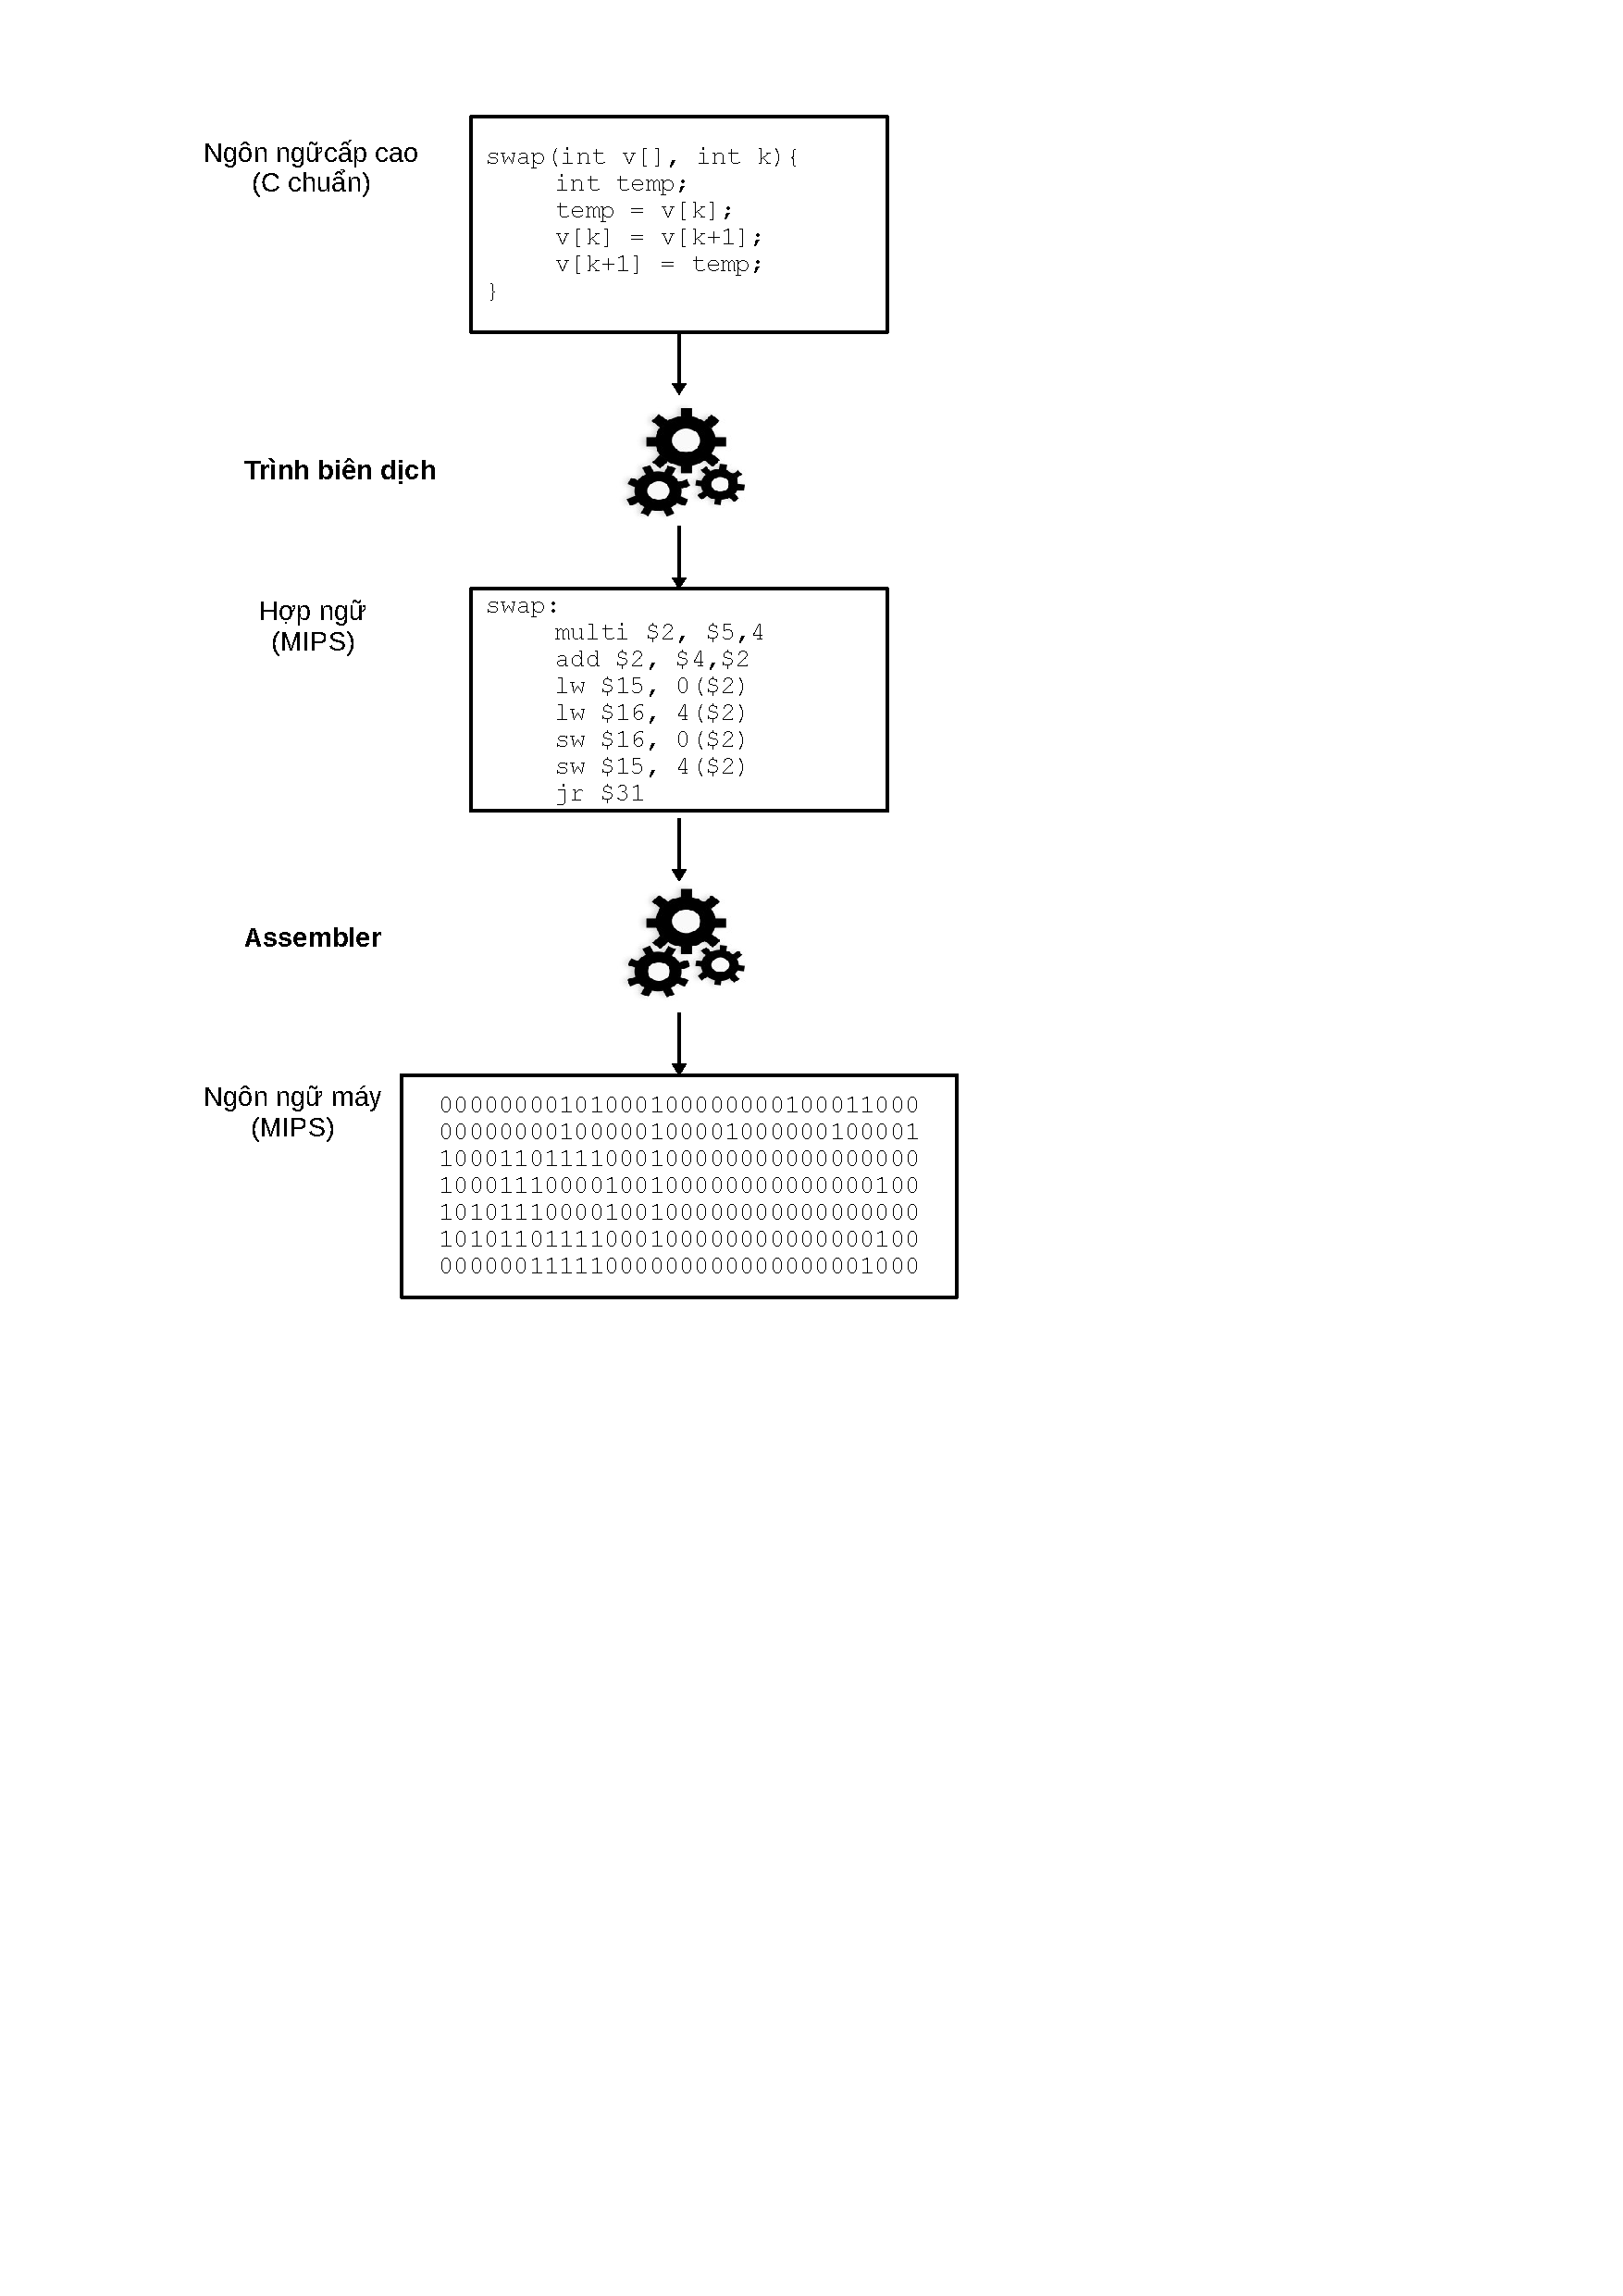
\includegraphics[width=0.75\columnwidth]{chapter01/figure/abstraction}
		\centering
	\caption{Các mức độ trừu tượng khác nhau của một chương trình. Ví dụ từ sách ``Computer Organization and Design: the Hardware/Software Interface.}
	\label{fig:abstraction}
\end{figure}

Hình \ref{fig:abstraction} trình bày mối quan hệ giữa các mức trừu tượng khác nhau. Ngày nay các ứng dụng thường được viết bằng ngôn ngữ lập trình cấp cao sau đó được biên dịch thành hợp ngữ bởi các trình biên dịch và cuối cùng được chuyển thành mã máy bởi trình hợp dịch.

\section{Công nghệ chế tạo bộ xử lý và bộ nhớ}

Phần~\ref{sec:history} đã giới thiệu các thế hệ máy tính khác nhau dựa trên những công nghệ sản xuất khác nhau. Ngày nay, tất cả các máy tính từ máy tính nhúng cho đến siêu máy tính cũng như các thiết bị điện tử từ đơn giản đến phức tạp đều được chế tạo bằng cách sử dụng công nghệ mạch tích hợp (integrated circuit). Các mạch tích hợp là các mạch điện tử chứa từ khoảng vài chục đến vài chục tỉ bóng bán dẫn (tại thời điểm năm 2016) kết nối với nhau theo một quy luật nào đó trên cùng một thiết bị (chip). Các mạch tích hợp đã và đang phát triển tuân theo định luật Moore. Sự gia tăng nhanh chóng số lượng bóng bán dẫn được tích hợp trên một chip dẫn đến sự gia tăng khả năng tính toán cho các bộ xử lý và gia tăng dung lượng bộ nhớ.

Quá trình sản xuất các mạch tích hợp bắt đầu với silicon, một loại vật liệu có thể tìm thấy trong cát. Bởi vì silicon không dẫn điện tốt cũng như không thật sự cách điện nên nó được gọi là \textbf{chất bán dẫn} (semiconductor). Ngành công nghiệp sản xuất mạch tích hợp sử dụng silicon như là thành phần chính nên còn được gọi là ngành công nghiệp bán dẫn. Trải qua quá trình hóa học đặc biệt, có thể thêm các vật liệu khác vào silicon để nó có thể có một trong ba đặc tính sau:
\begin{itemize}
\item Dẫn điện tốt - conductor (bằng cách thêm các dây đồng hoặc nhôm siêu nhỏ);
\item Cách điện hoàn toàn - insulator (giống như nhựa hoặc kính);
\item Có thể điều khiển dẫn hoặc không dẫn - transistor (giống như nhưng công tắc).
\end{itemize}
Một mạch tích hợp bao gồm sự kết hợp các phần tử thuộc ba dạng nói trên được chế tạo trên cùng một chip. Quy trình chế tạo các mạch tích hợp được tóm tắt như trong Hình~\ref{fig:IC_produce}.

\begin{figure}[!h]
	\centering
		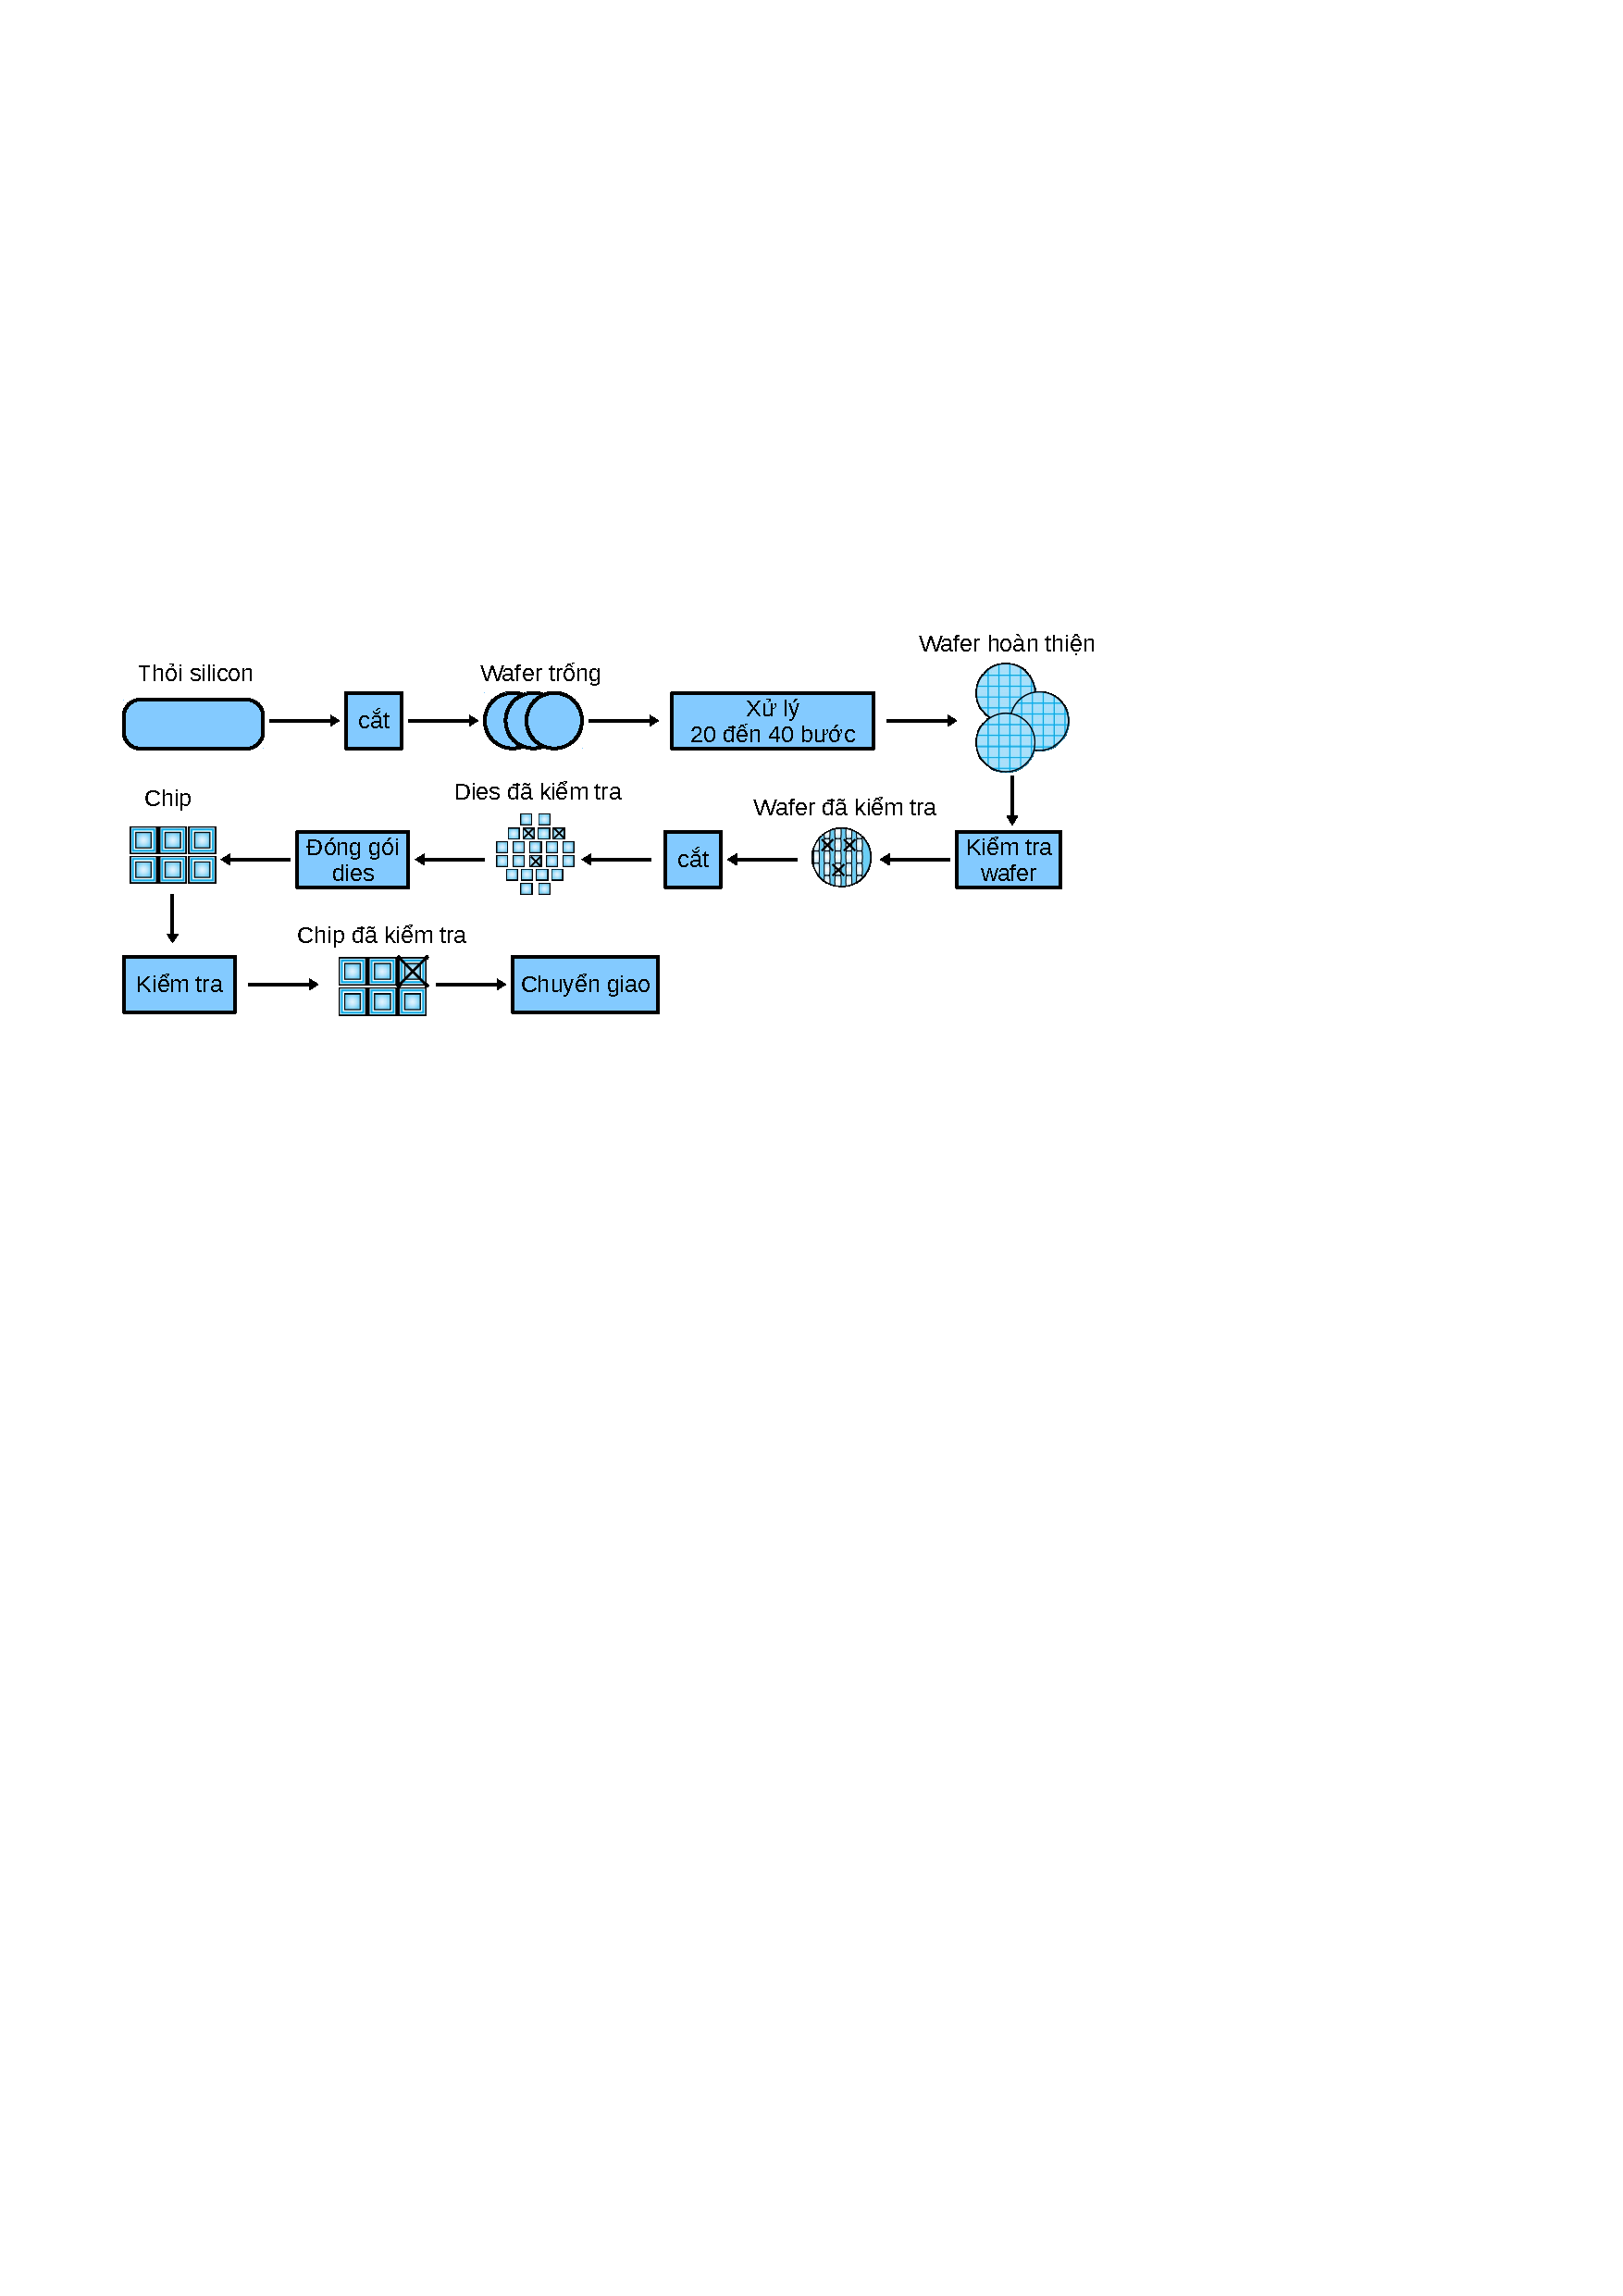
\includegraphics[width=1.0\columnwidth]{chapter01/figure/IC_produce}
		\centering
	\caption{Quy trình sản xuất các mạch tích hợp. Hình ảnh tham khảo từ sách ``Computer Organization and Design: the Hardware/Software Interface.}
	\label{fig:IC_produce}
	%\vspace{-1.0em}
\end{figure}

Quá trình chế tạo các mạch tích hợp bắt đầu từ một thỏi silicon nguyên chất có kích thước chiều dài khoảng từ 30 - 60 cm (12 - 24 inches) và chiều ngang khoảng 20 - 30 cm (8 - 12 inches). Thỏi silicon này sau đó sẽ được cắt ra thành các hình tròn với chiều dày khoảng 0.25 cm (0.1 inches) được gọi là các \emph{wafer}. Các wafer này sẽ được xử lý qua hàng loạt bước xử lý với những công nghệ và máy móc phức tạp để tạo thành các wafer hoàn thiện chứa các chip. Mỗi chip là một hình vuông/chữ nhật nhỏ trong wafer.

\begin{figure}[!h]
	\centering
		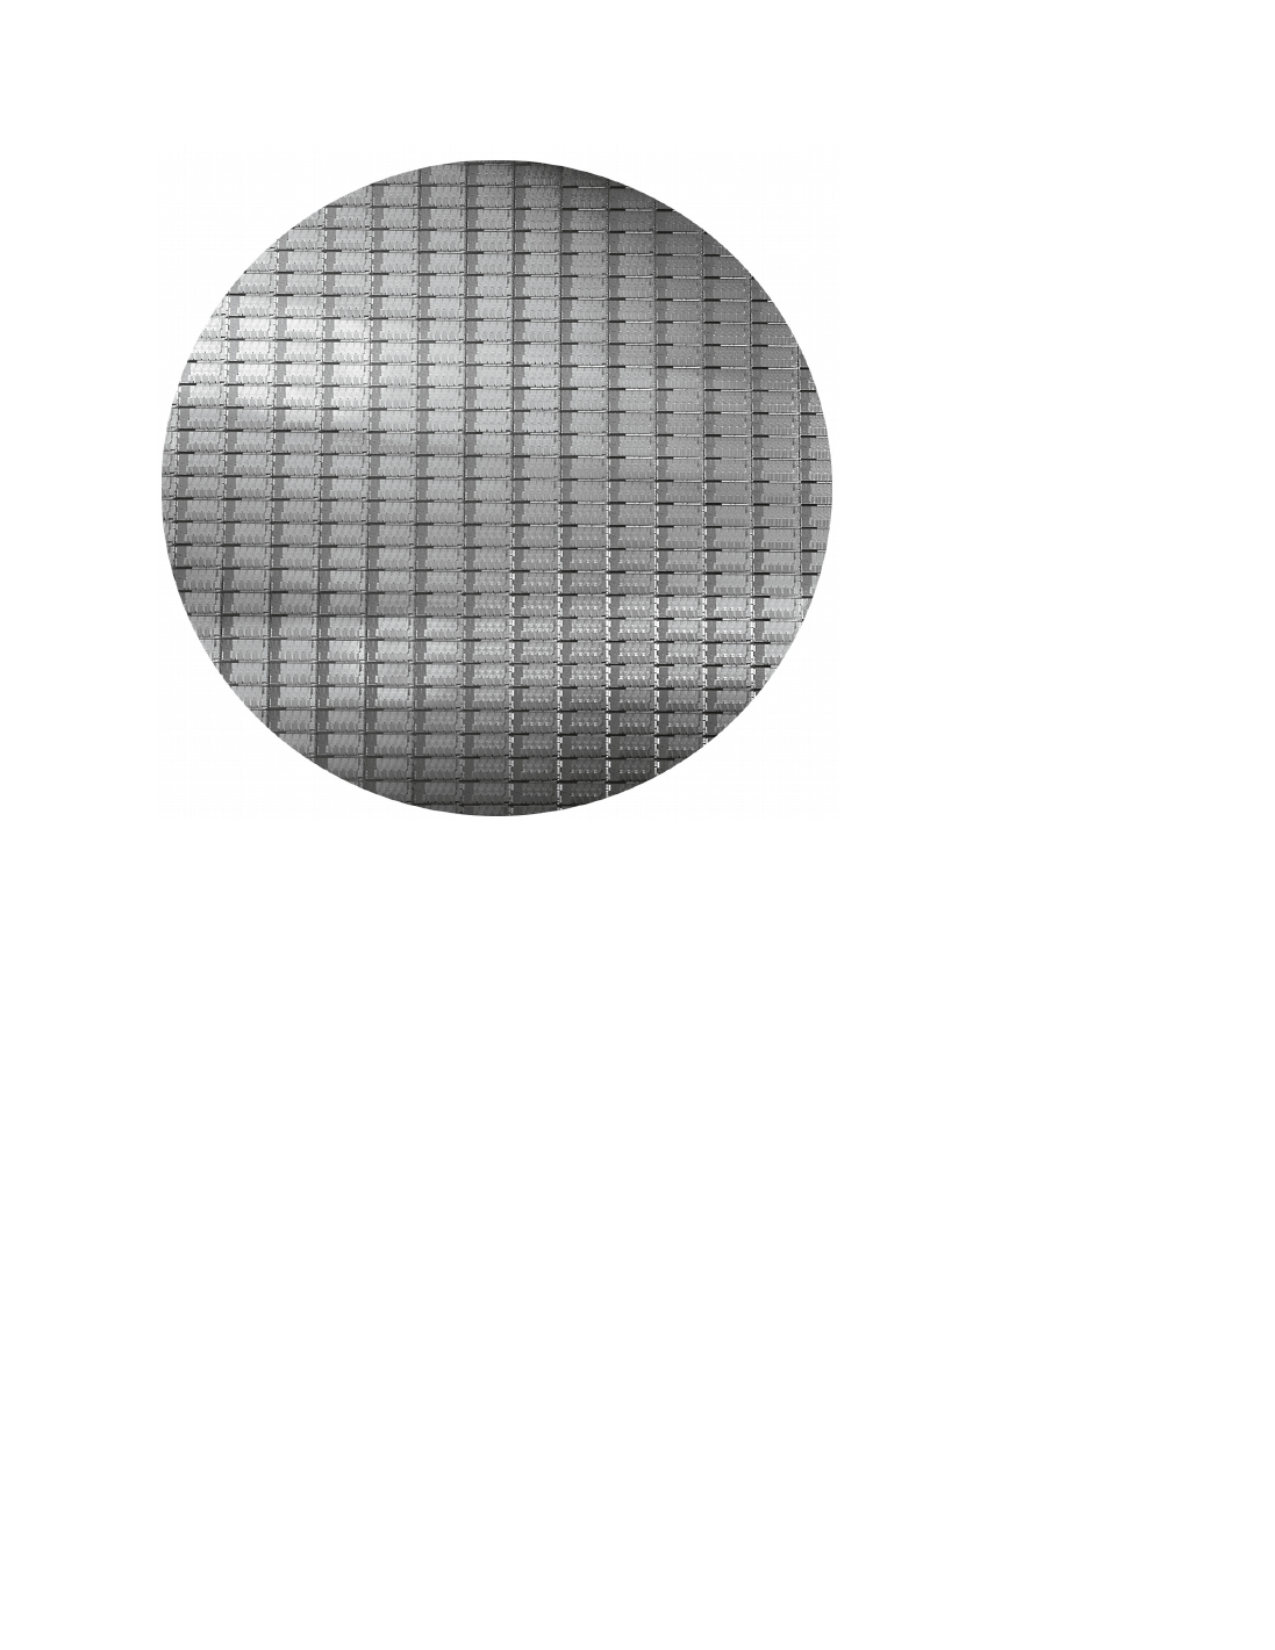
\includegraphics[width=0.5\columnwidth]{chapter01/figure/wafer}
		\centering
	\caption{Wafer khi sản xuất các chip Intel Core i7. Hình ảnh tham khảo từ sách ``Computer Organization and Design: the Hardware/Software Interface.}
	\label{fig:wafer}
\end{figure}

Hình~\ref{fig:wafer} là hình ảnh thực tế một wafer khi sản xuất các bộ xử lý Intel Core i7. Wafer này có đường kính 300 mm và mỗi chip có kích thước \mbox{20.7 $\times$ 10.5 mm}. Các wafer này sau đó sẽ được kiểm tra để đánh dấu các chip hư hỏng do quá trình sản xuất. Hư hỏng có thể xảy ra do các bước xử lý gặp lỗi hoặc có thể do chỉ một hạt bụi bám vào. Wafer sau đó sẽ được cắt để tạo thành các \emph{die}. Ví dụ trong quy trình ở Hình~\ref{fig:IC_produce} một wafer được cắt ra thành 20 die, trong đó các die đánh dấu `x' là các die hư hỏng. Các die không hư hỏng sau đó sẽ được mang đi đóng gói để tạo thành các chip. Sau khi đóng gói các chip sẽ được kiểm tra một lần nữa để loại trừ những hư hỏng trong quá trình đóng gói. Cuối cùng các chip hoàn thiện sẽ được chuyển giao cho khách hàng.

Trong quá trình sản xuất, các die hư hỏng do nhiều nguyên nhân khác nhau như đã trình bày ở trên. Tỉ lệ số die không hư hỏng trên tổng số die chứa trong một wafer được gọi là \textbf{Yield}. Thông thường Yield của một quy trình sản xuất được tính theo Công thức~\ref{eq:yield}, trong đó $\alpha$ tùy thuộc vào công nghệ sản xuất (thông thường $\alpha$ = 4.0), \emph{Defect per area} là tỉ lệ hư hỏng trên một đơn vị diện tích, và \emph{Die area} là diện tích một die.
\begin{equation}
\label{eq:yield}
\text{Yield} = (1 + \frac{\text{Defect per area} \times \text{Die area}}{\alpha})^{-\alpha}
\end{equation}

Trên một wafer sẽ có những die không nguyên vẹn do wafer hình tròn trong khi các die có hình vuông/chữ nhật. Các die ở phần rìa của wafer sẽ không nguyên vẹn và sẽ không thể sử dụng. Do đó, số lượng die trên một wafer, \emph{Die per wafer}, được tính theo Công thức~\ref{eq:die_exact}:
\begin{equation}
\label{eq:die_exact}
	\text{Die per wafer} = \frac{\pi d^2}{4S} - \frac{\pi d}{\sqrt{2S}}
\end{equation}
Trong đó, $d$ là đường kính wafer và $S$ là diện tích một die (\emph{die area}). Giá trị $\pi d/\sqrt{2S}$ là phần diện tích của những die không nguyên vẹn ở rìa wafer. Những die này không phải là một die hoàn chỉnh nên phải bị bỏ đi.

Tuy nhiên, tổng số die thu được từ một wafer, \emph{Die per wafer}, có thể được tính xấp xỉ theo Công thức~\ref{eq:die}.
\begin{equation}
\label{eq:die}
\text{Die per wafer} \approx \frac{\text{Wafer area}}{\text{Die area}} = \frac{\pi d^2}{4S}
\end{equation}

Giá thành sản xuất một die, \emph{Cost per die}, được tính dựa vào giá thành sản xuất wafer, \emph{Cost per wafer}, số lượng die thu được trên một wafer, và tỉ lệ die không hư hỏng theo Công thức~\ref{eq:die_cost}:
\begin{equation}
\label{eq:die_cost}
\text{Cost per die} = \frac{\text{Cost per wafer}}{\text{Die per wafer} \times \text{Yield}}
\end{equation}

Kích thước các wafer là cố định và giá thành sản xuất một wafer cũng thường cố định. Giá thành sản xuất một mạch tích hợp (một die) sẽ tăng khi kích thước mạch tích hợp tăng bởi vì hai nguyên nhân chính là số lượng die trên một wafer sẽ giảm và tỉ lệ hư hỏng sẽ tăng theo sự gia tăng của kích thước die. Do đó, để giảm giá thành sản xuất các mạch tích hợp thì cần giảm kích thước các die. Kích thước các die phụ thuộc vào kiến trúc và thiết kế mạch mà nó hiện thực cũng như công nghệ được dùng để chế tạo mạch. Các công nghệ chế tạo sử dụng kích thước bóng bán dẫn và dây dẫn nhỏ hơn liên tục được nghiên cứu đưa vào sử dụng để làm giảm giá thành. Ví dụ, các chip Intel Core i7 được sản xuất năm 2012 sử dụng công nghệ 32 nm, tức là kích thước của các bóng bán dẫn là 32 nm. Đến tháng 8 năm 2015, chip Intel Core i7 thế hệ thứ 6 được sản xuất bằng công nghệ 14 nm. Hình~\ref{fig:wafer} minh họa một tấm wafer chứa các chip Intel Core i7 năm 2012 sản xuất theo công nghệ 32 nm.

\begin{exmp}
\hrulefill\\
Tính giá thành sản xuất một chip Intel Core i7 theo công nghệ 32 nm, giả sử rằng để chế tạo một wafer Intel Core i7 như trong Hình~\ref{fig:wafer} sẽ tốn \$500 và tỉ lệ hư hỏng trên một cm$^2$ là 0.7.
\end{exmp}
\begin{answ}
Áp dụng Công thức~\ref{eq:die_exact} có thể tính được số lượng chip Intel Core i7 thu được trên một wafer là:
\begin{equation*}
\text{Die per wafer} = \frac{\pi d^2}{4S} - \frac{\pi d}{\sqrt{2S}} = \frac{\pi \times 30^2}{4 \times 2.07 \times 1.05} - \frac{\pi \times 30}{\sqrt{2 \times 2.07 \times 1.05}} \approx 280 \text{(die)}
\end{equation*}
Với tỉ lệ hư hỏng trên một $cm^2$ là $0.7$ ta có:
\begin{align*}
\text{Yield} &= (1 + \frac{\text{Defect per area} \times \text{Die area}}{\alpha})^{-\alpha} \\
	&= (1 + \frac{0.7 \times 2.07 \times 1.05}{4.0})^{-4.0} \approx 0.275
\end{align*}
Do đó, giá thành một chip Intel Core i7 chưa đóng gói (die) là:
\begin{equation*}
\text{Cost per die} = \frac{\text{Cost per wafer}}{\text{Die per wafer} \times\text{Yield}} \approx \frac{\$500}{280 \times 0.275} \approx \$6.494
\end{equation*}
\hrule
\end{answ}

\section{Hiệu suất và công suất}
Hiệu suất của một quá trình, một hệ thống sẽ đặc trưng cho ``độ lợi'' hay sức mạnh của hệ thống đó. Hiệu suất của các máy tính là yếu tố duy nhất dùng để so sánh khả năng xử lý của các máy tính khác nhau. Trong khi đó, công suất tiêu thụ là một trong những yếu tố có ảnh hưởng đến phương pháp cải tiến hệ thống máy tính nhằm tăng hiệu suất.

\subsection{Định nghĩa hiệu suất và tính toán hiệu suất}
\label{subsec:performance}
Khi lựa chọn một máy tính, yếu tố hiệu suất là một trong những thuộc tính quan trọng để lựa chọn. Do đó, đo đạc và so sánh chính xác hiệu suất giữa các máy tính là một đòi hỏi đối với người mua máy tính và cả người thiết kế máy tính. Hiểu được cách tốt nhất để đánh giá hiệu suất máy tính và các hạn chế trong đo hiệu suất là một điểm quan trọng trong việc lựa chọn máy tính.

Khi thực thi một chương trình trên hai máy tính cá nhân khác nhau, có thể khẳng định rằng máy tính nào hoàn thành chương trình nhanh hơn thì sẽ nhanh hơn. Do đó, đối với máy tính cá nhân, có thể sử dụng đại lượng \emph{\bfseries thời gian đáp ứng} (response time), còn được gọi là \emph{\bfseries thời gian thực thi} (execution time), để đánh giá máy tính. \emph{Thời gian đáp ứng} hay \emph{thời gian thực thi} là tổng thời gian mà một máy tính cần thiết để hoàn thành một tác vụ cụ thể bao gồm thời gian truy xuất đĩa, thời gian truy xuất bộ nhớ, thời gian đáp ứng các thiết bị ngoại vi, thời gian xử lý của hệ điều hành, thời gian CPU thực thi,...

Đối với một server hay một trung tâm xử lý dữ liệu (data center), cùng một thời điểm sẽ có nhiều người sử dụng và nhiều ứng dụng yêu cầu được xử lý. Do đó, máy tính nhanh hơn trong trường hợp này là máy tính có thể hoàn thành xử lý được nhiều ứng dụng hơn trong một đơn vị thời gian; ví dụ một ngày hay một giờ. Số lượng tác vụ máy tính hoàn thành trong một đơn vị thời gian được gọi là \emph{\bfseries lưu lượng} (throughput) hay \emph{\bfseries băng thông} (bandwidth). Đối với server hay các máy tính dùng cho trung tâm xử lý dữ liệu thì đại lượng \emph{lưu lượng} hay \emph{băng thông} thường được dùng để đánh giá máy tính.

\subsubsection{Mối quan hệ giữa thời gian thực thi và lưu lượng}
Khi thay thế bộ xử lý trong một máy tính bằng một bộ xử lý nhanh hơn, tức là làm giảm thời gian thực thi một chương trình. Bởi vì thời gian thực thi chương trình giảm đi so với bộ xử lý cũ nên số lượng chương trình được xử lý trong một đơn vị thời gian sẽ tăng lên. Do đó, lưu lượng hay băng thông của máy tính tăng. Ngược lại khi thay bộ xử lý cũ bằng bộ xử lý mới cùng tốc độ nhưng có nhiều lõi (core) hơn thì không làm thay đổi thời gian thực thi một chương trình vì một chương trình chỉ được thực thi trên một lõi. Tuy nhiên, bởi vì bộ xử lý có nhiều lõi có thể hoạt động song song nên trong một đơn vị thời gian số lượng chương trình được xử lý tăng so với bộ xử lý cũ. Điều này có nghĩa là lưu lượng hay băng thông của máy tính tăng. Nếu xét thời gian thực thi của hệ thống bằng thời gian thực thi của nhiều ($n$) ứng dụng thì thời gian thực thi sẽ giảm vì tại cùng một thời điểm có nhiều ứng dụng được thực thi xong xong. Do đó, tổng thời gian cần thiết thực thi $n$ ứng dụng sẽ giảm. Từ đây có thể kết luận rằng, trong các hệ thống máy tính thực thì hai đại lượng \emph{thời gian thực thi} và \emph{lưu lượng} có ảnh hưởng lẫn nhau.

\subsubsection{Định nghĩa và so sánh hiệu suất}
Hiệu suất (performance) của một hệ thống máy tính là đại lượng dùng để so sánh khả năng của các máy tính. Một cách đơn giản có thể nhận thấy rằng muốn tăng hiệu suất của máy tính thì chúng ta cần giảm thời gian thực thi. Do đó, hiệu xuất của một máy tính A được định nghĩa và tính toán bằng Công thức~\ref{eq:performance}:
\begin{equation}
\label{eq:performance}
\text{Performance}_A = \frac{1}{{\text{Execution time}}_A}
\end{equation}

Nếu máy tính A nhanh hơn (mạnh hơn) máy tính B thì ta có mối quan hệ giữa hai hiệu suất của hai máy tính A và B là:
\begin{align*}
\text{Performance}_A &> \text{Performance}_B\\
\Leftrightarrow \frac{1}{\text{Execution time}_A} &> \frac{1}{\text{Execution time}_B}\\
\Leftrightarrow {\text{Execution time}_A} &< {\text{Execution time}_B}
\end{align*}
Điều này có nghĩa là nếu máy tính A nhanh hơn máy tính B thì thời gian thực thi của máy B sẽ lớn hơn của máy A khi hai máy cùng xử lý một ứng dụng trong điều kiện giống nhau.

Trong thiết kế máy tính, chúng ta thường so sánh một cách định lượng hiệu suất của hai máy tính. Nếu phát biểu rằng ``máy tính A nhanh hơn máy tính B $n$ lần'' hay ``thời gian thực thi máy tính A nhỏ hơn thời gian thực thi máy tính B $n$ lần'' thì có nghĩa là:
\begin{equation*}
\frac{\text{Performance}_A}{\text{Performance}_B} = \frac{\text{Execution time}_B}{\text{Execution time}_A} = n
\end{equation*}


\begin{exmp}
\hrulefill\\
Nếu máy tính A thực thi một chương trình trong 10 s và máy tính B thực thi chương trình đó trong 20 s, hỏi máy tính A nhanh hơn máy tính B bao nhiêu lần?
\end{exmp}
\begin{answ}
Áp dụng công thức so sánh hiệu suất ta có:
\begin{equation*}
\frac{\text{Performance}_A}{\text{Performance}_B} = \frac{\text{Execution time}_B}{\text{Execution time}_A} = \frac{20}{10} = 2
\end{equation*}
Tức là máy tính A nhanh hơn máy tính B 2 lần; hay cũng có thể nói máy tính B chậm hơn máy tính A 2 lần.\\
\hrule
\end{answ}

\subsubsection{Tính toán hiệu suất thông qua thời gian}
Thời gian xử lý là phương tiện để đo đạc hiệu suất. Máy tính nào cần ít thời gian nhất để xử lý một công việc xác định sẽ là máy tính nhanh nhất, có hiệu suất cao nhất. Cách đơn giản nhất để đo thời gian xử lý một công việc xác định là dùng đại lượng \emph{thời gian thực thi} như đã giới thiệu ở trên hay còn được gọi là \emph{thời gian đáp ứng} hoặc \emph{\bfseries thời gian tổng thể} (elapsed time). Các đại lượng này là tổng thời gian cần thiết để hoàn thành một chương trình bao gồm: thời gian truy xuất đĩa, thời gian truy xuất bộ nhớ, thời gian đáp ứng các thiết bị nhập/xuất (I/O), thời gian phí tổn hệ điều hành,...

Tuy nhiên, có một thực tế rằng máy tính cùng một lúc sẽ xử lý nhiều ứng dụng khác nhau. Máy tính thường cố gắng tối ưu đại lượng số lượng tác vụ được xử lý trong một đơn vị thời gian hơn là tối ứng thời gian thực thi cho một ứng dụng. Ngoài ra thời gian đáp ứng các thiết bị nhập xuất còn phụ thuộc vào loại thiết bị và đôi khi phụ thuộc vào người sử dụng; thời gian phí tổn hệ điều hành tùy thuộc vào trạng thái và loại hệ điều hành,... Do đó, cần phân biệt được thời gian tổng thể và thời gian bộ xử lý thực sự xử lý chương trình. Thời gian bộ xử lý trung tâm (CPU) cần thiết để tính toán và xử lý chương trình được gọi là \emph{\bfseries thời gian thực thi CPU} (CPU execution time) hoặc đơn giản hơn là \emph{\bfseries thời gian CPU} (CPU time). Thời gian CPU không bao gồm thời gian chờ thiết bị ngoại vi hoặc thời gian xử lý ứng dụng khác. Tương tự, khi đề cập đến hiệu suất chúng ta cũng sẽ phân biệt hai loại hiệu suất đó là hiệu suất dựa trên thời gian tổng thể (còn được gọi là \emph{hiệu suất hệ thống} - system performance)và hiệu suất dựa trên thời gian CPU (còn được gọi lạ \emph{hiệu suất CPU} - CPU performance).

Đối với người sử dụng máy tính thì thời gian thực thi là đại lượng được quan tâm. Tuy nhiên đối với người thiết kế máy tính thì đại lượng \textbf{chu kỳ xung nhịp} (clock cycle) được quan tâm hơn vì hầu hết các máy tính đều hoạt động đồng bộ với \emph{xung nhịp} (clock). Xung nhịp là đại lượng biểu thị cho tốc độ xử lý của các khối chức năng phần cứng. Độ dài xung nhịp được tính toán bằng thời gian chu kỳ (cycle), ví dụ 250 ps, hay bằng \textbf{tần số} (frequency, clock rate). Tần số xung nhịp được tính bằng nghịch đảo của chu kỳ xung nhịp và có đơn vị là Hz, ví dụ 4 GHz (gigahertz). Tần số xung nhịp là số chu kỳ xung nhịp trong một giây.

Giữa thời gian thực thi CPU hay thời gian CPU của một chương trình và chu kỳ (tần số) xung nhịp đồng bộ của CPU có mối quan hệ với nhau. Biểu thức~\ref{eq:time_cycle} biểu diễn mối quan hệ này. Thời gian CPU cho một chương trình bằng tổng số chu kỳ xung nhịp cần thiết để thực thi chương trình (CPU clock cycles) nhân với thời gian một chu kỳ xung nhịp (Clock cycle time). Bởi vì thời gian một chu kỳ xung nhịp bằng nghịch đảo của tần số xung nhịp nên thời gian thực thi một chương trình bằng số lượng chu kỳ xung nhịp cần thiết cho chương trình chia cho tần số xung nhịp (clock rate).
\begin{align}
\label{eq:time_cycle}
\text{CPU time} &= \text{CPU clock cycles} \times \text{Clock cycle time} \nonumber\\
 &= \frac{\text{CPU clock cycles}}{\text{Clock frequency}}
\end{align}

Từ Biểu thức~\ref{eq:time_cycle} có thể thấy rằng, để tăng hiệu suất của một máy tính, hay giảm thời gian CPU của một chương trình trên máy tính đó thì hoặc là cần giảm số lượng chu kỳ cần thiết cho chương trình đó hoặc là giảm thời gian một chu kỳ xung nhịp (tăng tần số xung nhịp). Tuy nhiên, việc giảm thời gian một chu kỳ xung nhịp hay tăng tần số xung nhịp thường làm gia tăng số lượng chu kỳ cần thiết để xử lý chương trình. Các chương tiếp theo sẽ phân tích kỹ hơn vấn đề này.

\begin{exmp}
\hrulefill\\
Máy tính A hoạt động ở tần số 2 GHz thực thi một chương trình trong 10 s. Các kỹ sư muốn thiết kế một máy tính B có khả năng thực thi chương trình đó chỉ trong thời gian 7 s bằng cách tăng tần số so với máy tính A. Tuy nhiên, khi tăng tần số thì số chu kỳ cần thiết để thực thi chương trình trên máy B cũng tăng lên 1.4 lần so với số chu kỳ cần thiết để thực thi chương trình trên máy tính A. Hỏi tần số máy tính B phải là bao nhiêu để đạt được thời gian xử lý như mong muốn. 
\end{exmp}
\begin{answ}
Áp dụng công thức mối quan hệ giữa thời gian thực thi và tần số xung nhịp ta có:
\begin{align*}
\text{CPU time}_A &= \frac{\text{CPU clock cycles}_A}{\text{clock rate}_A}\\
\text{CPU time}_B &= \frac{\text{CPU clock cycles}_B}{\text{clock rate}_B}\\
\implies \frac{\text{CPU time}_A}{\text{CPU time}_B} &= \frac{\text{CPU clock cycles}_A}{\text{CPU clock cycles}_B} \times \frac{\text{clock rate}_B}{\text{clock rate}_A} \\
\implies \text{clock rate}_B &= \frac{\text{CPU time}_A}{\text{CPU time}_B} \times \frac{\text{CPU clock cycles}_B}{\text{CPU clock cycles}_A} \times \text{clock rate}_A \\
\Leftrightarrow \text{clock rate}_B &= \frac{10\text{ s}}{7\text{ s}} \times 1.4 \times 2\text{ GHz} = 4\text{ GHz}
\end{align*}
\hrule
\end{answ}

\subsubsection{Tính toán hiệu suất thông qua số lệnh}
Vấn đề nảy sinh ở đây là làm sao đếm được số chu kỳ xung nhịp cần thiết cho một đoạn chương trình? Tính toán hiệu suất thông qua thời gian thực thi CPU không đề cập đến số lượng lệnh của chương trình. Tuy nhiên, một chương trình sau khi được biên dịch sẽ gồm những lệnh và những lệnh này sẽ được máy tính thực thi. Do đó, thời gian thực thi một chương trình phụ thuộc vào số lượng lệnh của chương trình. Thời gian thực thi chương trình sẽ là tích của thời gian thực thi trung bình một lệnh và tổng số lệnh của chương trình (Instruction count). Nếu thời gian thực thi được đo dựa vào số chu kỳ thì số chu kỳ cần thiết cho một chương trình được tính theo Công thức~\ref{eq:cpu_cycles}.
\begin{equation}
\label{eq:cpu_cycles}
\text{CPU clock cycles} = \text{Instructions count}\times\text{Clock cycles per instruction}
\end{equation}
Trong đó đại lượng \emph{số chu kỳ trên một lệnh} (Clock cycles per instruction) là số lượng chu kỳ trung bình cần thiết để hoàn thành một lệnh. Đại lượng số chu kỳ trên một lệnh thường được gọi là \textbf{CPI} của một chương trình hay một đoạn chương trình. Do các lệnh khác nhau sẽ thực thi những công việc khác nhau, ví dụ lệnh nhân và lệnh cộng, nên thời gian để hoàn thành các lệnh cũng sẽ khác nhau. Do đó, đại lượng CPI được tính bằng giá trị trung bình của tất cả các lệnh trong một chương trình hoặc một đoạn chương trình. CPI thường được dùng để so sánh các hiện thực phần cứng khác nhau hỗ trợ cùng một kiến trúc tập lệnh (Instruction Set Architecture - ISA) bởi vì số lượng lệnh khi sử dụng cùng một kiến trúc tập lệnh cho một chương trình là như nhau.

\begin{exmp}
\hrulefill\\
Một tập lệnh cùng được hiện thực cho hai máy tính khác nhau, máy A và máy B. Máy A có thể hoạt động ở tần số 4 GHz trong khi máy B chỉ hoạt động được ở tần số 2 GHz. Khi thực thi một chương trình trên máy A người ta đo được giá trị CPI là 2.0 trong trên máy B là 1.2. Hỏi máy nào thực thi chương trình này nhanh hơn và nhanh hơn bao nhiêu?
\end{exmp}
\begin{answ}
Bởi vì hai máy cùng hiện thực một tập lệnh nên số lượng lệnh cần thiết cho chương trình trên cả hai máy là giống nhau. Gọi giá trị này là \emph{IC}.

Áp dụng Công thức~\ref{eq:cpu_cycles} ta có tổng số chu kỳ cần thiết để các máy hoàn thành chương trình lần lượt là:
\begin{align*}
\text{CPU clock cycles}_A &= \text{IC} \times \text{CPI}_A\\ 
\text{CPU clock cycles}_B &= \text{IC} \times \text{CPI}_B
\end{align*}

Bởi vì thời gian thực thi chương trình sẽ bằng số lượng chu kỳ cần thiết chia cho tần số nên ta có thời gian thực thi chương trên hai máy A và B lần lượt là:
\begin{align*}
\text{CPU time}_A &= \frac{\text{IC} \times \text{CPI}_A}{\text{frequency}_A} = \frac{\text{IC} \times 2.0}{4\times 10^9} = \text{IC} \times 500\text{ ps}\\ 
\text{CPU time}_B &= \frac{\text{IC} \times \text{CPI}_B}{\text{frequency}_B} = \frac{\text{IC} \times 1.2}{2\times 10^9} = \text{IC} \times 600\text{ ps}
\end{align*}
Rõ ràng, máy tính A sẽ thực thi chương trình nhanh hơn máy tính B 1.2 lần.\\
\hrule
\end{answ}

Từ ví dụ trên có thể thấy rằng thời gian CPU có thể được tính thông qua CPI, số lượng lệnh của chương trình và chu kỳ xung nhịp hoặc tần số xung nhịp bằng Công thức~\ref{eq:cpu_time}:
\begin{align}
\label{eq:cpu_time}
	\text{CPU time} &= \text{CPU clock cycles} \times \text{Clock cycle time} \nonumber \\
	&= \text{Instruction count}\times \text{CPI} \times \text{Clock cycle time}  \\
	& = \frac{\text{Instruction count}\times \text{CPI}}{\text{clock rate}} \nonumber
\end{align}

Công thức~\ref{eq:cpu_time} thường được sử dụng để tính toán thời gian CPU cần thiết để thực thi một chương trình bởi vì nó phản ánh ba yếu tố chính ảnh hưởng đến hiệu suất của máy tính đó là \emph{số lượng lệnh}, \emph{CPI}, và \emph{tần số}. Thời gian thực thi tỉ lệ thuận với số lượng lệnh và CPI trong khi tỉ lệ nghịch với tần số xung nhịp. Công thức này thường dược dùng so sánh các hiện thực khác nhau hoặc đánh giá các thiết kế khác nhau khi biết được ba yếu tố này.

\begin{exmp}
\label{exmp:compiler}
\hrulefill\\
Một máy tính có ba loại lệnh A, B, và C lần lượt có CPI cho từng loại lệnh là 1, 2, và 3. Có hai chương trình dịch cùng dịch một đoạn chương trình ở ngôn ngữ cấp cao thành các lệnh thuộc ba loại lệnh trên. Số lượng lệnh cho mỗi loại ứng với từng chương trình dịch như sau:
\begin{table}[h]
\centering
		\begin{tabular}{c||C{1.0cm}|C{1.0cm}|C{1.0cm}}
			\hline
			\multirow{2}{*}{\textbf{Chương trình dịch}} & \multicolumn{3}{c}{\textbf{Số lượng lệnh các loại}} \\
			\cline{2-4}
			& A & B & C\\
			\hline
			\hline
			1 & 2 & 4 & 2 \\
			\hline
			2 & 4  & 1 & 1 \\
			\hline
		\end{tabular}
\end{table}

Đoạn chương trình được dịch bởi chương trình dịch nào sẽ có thời gian thực thi nhanh hơn? Giá trị CPI trung bình cho từng đoạn chương trình được dịch bởi các chương trình dịch khác nhau là bao nhiêu?
\end{exmp}

\begin{answ}
Tổng số lượng chu kỳ cần thiết cho một đoạn chương trình sẽ bằng tổng số chu kỳ cần thiết cho các lệnh thuộc các nhóm lệnh khác nhau. Do đó, ta có thể tính số chu kỳ cần thiết cho một đoạn chương trình như sau:
\begin{equation*}
\text{CPU clock cycles} = \sum_{i = 1}^{n} (\text{CPI}_i \times \text{IC}_i)
\end{equation*}
Trong đó $\text{IC}_i$ là số lượng lệnh loại $i$ trong đoạn chương trình và $\text{CPI}_i$ là CPI của loại lệnh $i$.

Như vậy, tổng số chu kỳ xung nhịp cần thiết để xử lý hai đoạn chương trình trên lần lượt là:
\begin{align*}
\text{CPU clock cycles}_1 &= \sum_{i = 1}^{n} (\text{CPI}_i \times \text{IC}_i) = 2 \times 1 + 1 \times 2 + 2 \times 3 = \text{10 (chu kỳ)}\\
\text{CPU clock cycles}_2 &= \sum_{i = 1}^{n} (\text{CPI}_i \times \text{IC}_i) = 4 \times 1 + 1 \times 2 + 1 \times 3 = \text{9 (chu kỳ)}
\end{align*}
Đoạn chương trình được dịch bởi chương trình dịch 2 sẽ có thời gian thực thi nhanh hơn đoạn chương trình được dịch bởi trình dịch 1. Hay chương trình dịch 2 tốt hơn chương trình dịch 1 khi dịch ứng dụng cụ thể này.

CPI trung bình của các đoạn chương trình sẽ bằng tổng số chu kỳ cần thiết để thực thi đoạn chương trình chia cho số lượng lệnh trong đoạn chương trình đó. Do đó, giá trị CPI trung bình của hai đoạn chương trình trên lần lượt là:
\begin{align*}
\text{CPI}_1 &= \frac{\text{CPU clock cycles}_1}{\text{Instruction count}_1} = \frac{10}{5} = 2.0\\
\text{CPI}_2 &= \frac{\text{CPU clock cycles}_2}{\text{Instruction count}_2} = \frac{9}{6} = 1.5
\end{align*}

Trong trường hợp này CPI$_2$ < CPI$_1$ và tương đồng với kết quả chương trình dịch 2 tốt hơn chương trình dịch 1. Tuy nhiên, chỉ dựa vào yếu tố CPI không thể kết luận được điều này. Ví dụ minh họa để dành cho người đọc.\\
\hrule
\end{answ}

Tổng kết lại, các yếu tố ảnh hưởng đến hiệu suất của một chương trình bao gồm: \emph{giải thuật}, \emph{ngôn ngữ lập trình}, \emph{trình biên dịch}, \emph{kiến trúc} và \emph{cấu trúc phần cứng}.

\subsection{Công suất và giới hạn công suất}
Hiện nay, hầu hết các mạch tích hợp đều được chế tạo với công nghệ đang chiếm ưu thế là CMOS (complementary metal oxide semiconductor). Công suất tiêu thụ (power) của các mạch tích hợp này sẽ bao gồm hai thành phần là \emph{công suất tĩnh} (static power) và \emph{công suất động} (dynamic power). Công suất tĩnh trong mạch tích hợp dùng công nghệ CMOS là công suất tiêu thụ của các bóng bán dẫn khi nó không hoạt động. Công suất tĩnh trong công nghệ CMOS thường nhỏ và có thể bỏ qua trong tính toán. Ngược lại, công suất động là công suất tiêu thụ khi các bóng bán dẫn thay đổi trạng thái (switching). Đây là nguồn tiêu thụ năng lượng chủ yếu trong các mạch tích hợp công nghệ CMOS. Công suất động phụ thuộc vào điện dung của các bóng bán dẫn ($C$), nguồn cung cấp ($V_{dd}$) và tần số thay đổi trạng thái ($f$) của các bóng bán dẫn. Công suất tiêu thụ của các mạch tích hợp theo công nghệ CMOS được xấp xỉ bằng công suất động và được tính theo Công thức~\ref{eq:power}.
\begin{equation}
\label{eq:power}
\text{Power} = C\times {V_{dd}}^2 \times f
\end{equation}

Tần số thay đổi trạng thái của các bóng bán dẫn chính là tần số hoạt động (clock rate) của mạch tích hợp. Điện dung của mạch tích hợp phụ thuộc vào công nghệ chế tạo và số lượng bóng bán dẫn trong mạch tích hợp. Do đó, nếu điện áp nguồn ($V_{dd}$) không đổi thì công suất tiêu thụ sẽ tăng tuyến tính với sự tăng tần số xung nhịp. Điều này cản trở sự phát triển của máy tính do công suất tiêu thụ càng lớn thì quá trình tản nhiệt làm mát hệ thống càng phức tạp.

Do đó, phải giảm công suất tiêu thụ bằng cách giảm điện áp nguồn cung cấp cho mạch tích hợp. Điều này có thể thực hiện được bằng cách tạo ra các thế hệ mạch tích hợp sử dụng các công nghệ tiên tiến hơn. Thông thường công nghệ mới ra đời sẽ giảm được khoảng 15\% điện áp nguồn. Trong hơn 20 năm qua, điện áp nguồn đã giảm từ 5 V xuống 1 V.

\begin{exmp}
\hrulefill\\
Giả sử thiết kế được một bộ xử lý đơn giản hơn bộ xử lý cũ nên điện dung giảm 15\%. Do sử dụng công nghệ mới nên điện áp nguồn cũng chỉ bằng 85\% điện áp nguồn trước đây. Bộ xử lý mới hoạt động ở tần số cao hơn bộ xử lý cũ 20\%. Hỏi công suất tiêu thụ bộ xử lý mới tăng hay giảm so với công suất tiêu thụ bộ xử lý cũ?
\end{exmp}
\begin{answ}
Áp dụng Công thức~\ref{eq:power} ta có mối quan hệ giữa công suất tiêu thụ của hai bộ xử lý:
\begin{equation*}
\frac{P_{new}}{P_{old}} = \frac{0.85C \times (0.85V_{dd})^2 \times 1.2f}{C \times V_{dd}^2 \times f} = 0.74
\end{equation*}
Vậy, công suất tiêu thụ bộ xử lý mới bằng 0.74 lần công suất tiêu thụ bộ xử lý cũ (giảm 26\%).\\
\hrule
\end{answ}

Tuy nhiên, vấn đề đang gặp phải hiện nay là không thể hạ thấp điện áp nguồn hơn nữa vì khi điện áp nguồn quá thấp thì các bóng bán dẫn sẽ không hoạt động chính xác. Do đó, vấn đề nâng cao tần số xung nhịp để tăng hiệu suất hoạt động của các mạch tích hợp nói chung và của các máy tính chế tạo theo công nghệ CMOS nói riêng đang gặp phải vấn đề về giới hạn công suất (power wall). Hình~\ref{fig:power} cho thấy mối quan hệ giữa công suất tiêu thụ và tần số xung nhịp của mười một thế hệ máy tính nổi tiếng của Intel trong hơn 30 năm qua. Cả tần số xung nhịp và công suất tiêu thụ đều tăng nhanh chóng trong những thập niên đầu và bắt đầu chững lại trong những năm gần đây do vấn đề giới hạn công suất.

\begin{figure}[!h]
	\centering
		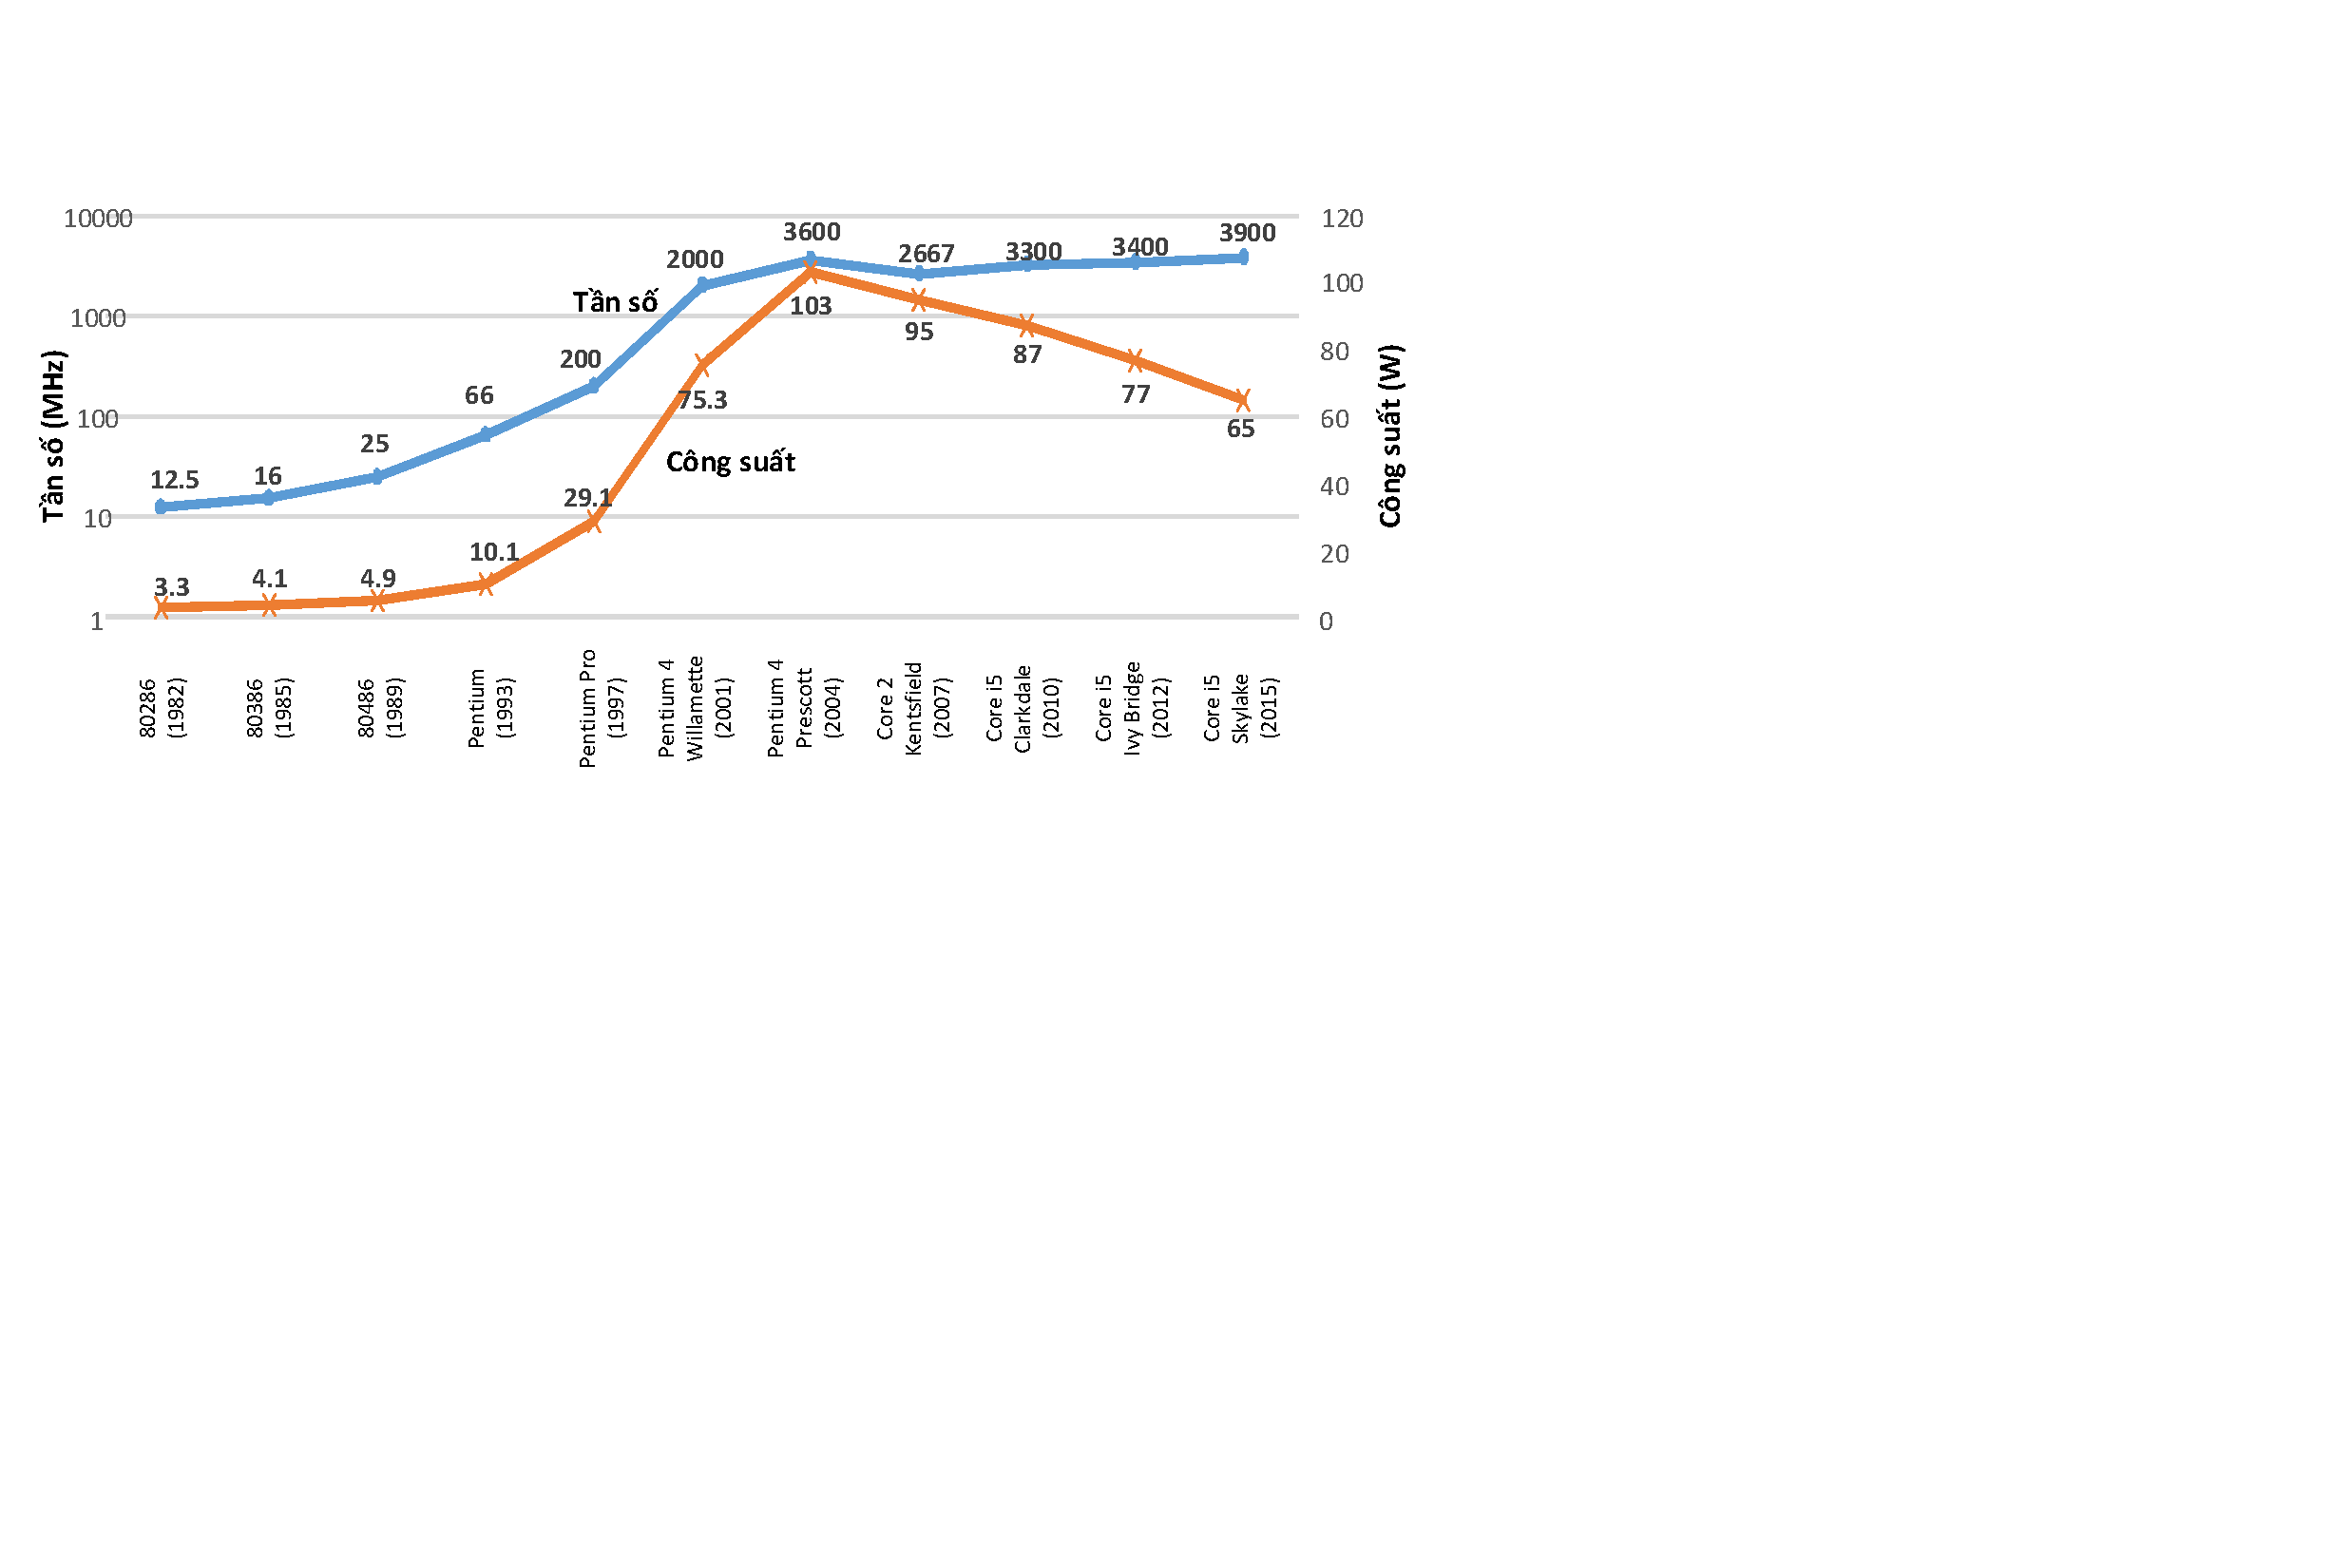
\includegraphics[width=0.95\columnwidth]{chapter01/figure/power}
		\centering
	\caption{Mối quan hệ giữa công suất tiêu thụ và tần số xung nhịp của mười một thế hệ máy tính x86 nổi tiếng của Intel. Nguồn số liệu http://www.intel.com}
	\label{fig:power}
\end{figure}

Để giải quyết vấn đề công suất tiêu thụ, các chip được đóng gói có kích thước lớn để dễ tản nhiệt và các chip có thể được tắt những phần không được sử dụng tại từng thời điểm. Mặc dù có nhiều công nghệ tản nhiệt khác nhau có thể áp dụng cho những chip có công suất tiêu thụ lớn hơn nhiều, ví dụ 300 watts, tuy nhiên các công nghệ này rất tốn kém và không thể áp dụng cho các máy tính cá nhân và đặc biệt là cho các thiết bị di động.

\section{Các lỗi sai thường gặp}

Trong thiết kế cũng như đánh giá máy tính, các lỗi sai sau đây thường xảy ra.

\begin{pitfall}
\emph{Có thể cải tiến một thành phần nào đó của một máy tính để tăng hiệu suất toàn máy tính một lượng tỉ lệ với phần cải tiến}
\end{pitfall}

Lỗi sai này có thể được chứng minh qua ví dụ sau và áp dụng định luật Amdahl. Giả sử rằng một chương trình thực thi trên một máy tính trong thời gian 50 giây, trong đó thời gian xử lý phép toán số thực chiếm 80\%. Câu hỏi đặt ra là phải cải tiến việc xử lý phép toán số thực bao nhiêu lần để thời gian xử lý của chương trình giảm đi 5 lần. Theo định luật Amdahl ta có mối quan hệ giữa thời gian thực thi trước và sau khi cải tiến như sau:
\begin{align*}
\text{Thời gian sau cải tiến} &= \frac{\text{Thời gian phần ảnh hưởng bởi cải tiến}}{\text{Tỉ lệ cải tiến}}\\ &+ \text{Thời gian phần không bị ảnh hưởng bởi cải tiến}
\end{align*}

Trong trường hợp này, thời gian phần ảnh hưởng bởi cải tiến là thời gian xử lý các phép toán số thực là 40 giây (chiếm 80\% thời gian thực thi chương trình), thời gian mong muốn sau cải tiến là 10 giây (cải tiến thời gian thực thi 5 lần), thời gian không ảnh hưởng bởi cải tiến tức là thời gian thực thi các phép toán khác phép toán số thực là 10 giây (50 giây - 40 giây = 10 giây). Do đó, áp dụng định luật Amdahl:
\begin{align*}
10 = \frac{40}{n} + 10
\end{align*}
Rõ ràng là không thể tìm được $n$, tức là không thể chỉ cải tiến phép tính số thực để có thể cải tiến thời gian thực thi toàn chương trình 5 lần.

\begin{pitfall}
\emph{Chỉ sử dụng một phần của công thức đánh giá hiệu suất để tính toán hiệu suất.}
\end{pitfall}

Như đã trình bày trong Phần~\ref{subsec:performance}, hiệu suất của một máy tính được tính toán thông qua ba tham số: \emph{tần số xung nhịp}, \emph{số lượng lệnh} và \emph{CPI}. Một trong những lỗi sai thường gặp là chỉ dùng một hoặc hai trong ba tham số trên để đánh giá hiệu suất của một máy tính. Một ví dụ thường thấy là dùng khái niệm \emph{số triệu lệnh trên một giây} (million instructions per second - MIPS) để so sánh hiệu suất của hai máy tính. MIPS được định nghĩa là số triệu lệnh máy tính thực hiện được trong một giây và được tính theo Công thức~\ref{eq:MIPS}:
\begin{align}
\label{eq:MIPS}
	\text{MIPS} &= \frac{\text{Instruction count}}{\text{Execution time}\times 10^6}
	= \frac{\text{Instruction count}}{\frac{\text{Instruction count} \times \text{CPI}}{\text{clock rate}}\times 10^6}
	= \frac{\text{clock rate}}{\text{CPI} \times 10^6}
\end{align}

Từ định nghĩa MIPS có thể thấy rằng máy tính nhanh hơn sẽ có MIPS lớn hơn. Tuy nhiên theo Công thức~\ref{eq:MIPS} thì MIPS chỉ phụ thuộc vào hai trong ba tham số đánh giá hiệu suất do đó sẽ gặp các vấn đề sau đây:
\begin{itemize}[-]
\item Nếu hai máy tính có tập lệnh khác nhau thì không thể dùng đại lượng MIPS để so sánh vì số lượng lệnh sẽ khác nhau;
\item MIPS phụ thuộc vào CPI và CPI của các chương trình khác nhau là khác nhau mặc dù trên cùng một máy tính, do đó một máy tính sẽ có nhiều giá trị MIPS tùy thuộc vào chương trình;
\item Một chương trình có thể được biên dịch ra nhiều lệnh hơn nhưng các lệnh này lại thực thi nhanh hơn (như trong Ví dụ~\ref{exmp:compiler}), do đó MIPS độc lập với hiệu suất.
\end{itemize}

\section{Kết chương}

Được ra đời vào năm 1946, máy tính điện tử đa dụng đã trải qua quá trình phát triển nhanh chóng cả về công nghệ chế tạo lẫn về năng lực tính toán. Mặc dù còn nhiều tranh cải nhưng sự phát triển của các thế hệ máy tính có thể chia thành bốn thế hệ dựa vào công nghệ chế tạo ra nó: thế hệ thứ nhất sử dụng đèn chân không, thế hệ thứ hai sử dụng các bóng bán dẫn, thế hệ thứ ba hình thành cùng với sự ra đời của mạch tích hợp và thế hệ máy tính thứ tư dùng công nghệ mạch tích hợp lớn.

Mạch tích hợp là cơ sở để phát triển các loại máy tính hiện tại từ siêu máy tính đến các máy tính nhúng. Công nghệ mạch tích hợp đã và đang phát triển nhanh chóng cả về kích thước các bóng bán dẫn lẫn số lượng các bóng bán dẫn được tích hợp trên cùng một chip. Tuy nhiên, hiệu suất của các máy tính phụ thuộc không chỉ vào tần số xung nhịp, được quyết định bởi kiến trúc của máy tính và công nghệ chế tạo, mà còn phụ thuộc vào hai đại lượng quan trọng khác là số chu kỳ trung bình mỗi lệnh (CPI) và số lượng lệnh của chương trình.

Trong thời gian gần đây, tần số xung nhịp của các máy tính hầu như không thể tăng do giới hạn công suất tiêu thụ của các chip. Do đó, xu hướng phát triển của các máy tính ngày nay là xu hướng đa xử lý và các bộ xử lý nhiều lỗi. Các vấn đề này sẽ được giới thiệu chi tiết ở các chương tiếp theo.

\section{Câu hỏi ôn tập và bài tập}
\begin{exer}
\label{exer:chip}
Cho bảng số liệu sau:
\begin{table}[h]
\centering
		\begin{tabular}{c||C{2cm}|C{2cm}|C{2cm}|C{2cm}}
		\hline
		\textbf{Chip} & \textbf{Kích thước chip (mm$^2$)} & \textbf{Tỉ lệ hư hỏng (cm$^2$)} & \textbf{Công nghệ sản xuất (nm)} & \textbf{Số triệu transistors/chip}\\
		\hline
		\hline
		IBM Power5 & 389 & 0.3 & 130 & 276\\
		\hline
		Sun Niagara & 380 & 0.75 & 90 & 279\\
		\hline
		AMD Operton & 199 & 0.75 & 90 & 233\\
		\hline
		\end{tabular}
\end{table}

\begin{enumerate}[a.]
\item Tính Yield của các loại chip nếu giả sử $\alpha=4$?
\item Tại sao Yield của chip Sun Niagara lại nhỏ hơn Yield của AMD Operton nhiều mặc dù cả hai có cùng tỉ lệ hư hỏng?
\end{enumerate}
\end{exer}

\begin{exer}
Giả sử rằng, một công ty đang chuẩn bị đầu từ dây chuyền sản xuất chip IBM Power5 (chip IBM Power5 cũ như trong Bài tập~\ref{exer:chip}). Phòng chiến lược của công ty dự báo rằng nếu đầu tư dây chuyền sản xuất mới thì cần đầu tư 1 tỉ USD. Sau khi đầu tư dây chuyền sản xuất mới xong thì số lượng chip bán ra trong mỗi tháng sẽ nhiều hơn hiện tại 3 lần và mỗi chip mới có thể bán với giá cao hơn chip cũ 2 lần. Biết rằng chip IBM Power5 sản xuất theo dây chuyền mới sẽ có kích thước là 185 mm$^2$, tỉ lệ hư hỏng là 0.7 trên mỗi cm$^2$. Giá thành sản xuất mỗi wafer đường kính 300 mm theo cả dây chuyền cũ lần mới đều là 500 USD. Hiện tại giá bán mỗi chip IBM Power5 cao hơn giá thành sản xuất là 40\%.
\begin{enumerate}[a.]
\item Tính giá thành sản xuất chip IBM Power5 cũ và mới?
\item Tính lợi nhuận của mỗi chip IBM Power5 cũ và mới?
\item Nếu hiện tại mỗi tháng bán được 500.000 chip IBM Power5, cần bao nhiêu tháng để có thể thu hồi vốn đầu tư cho dây chuyền sản xuất mới?
\end{enumerate}
\end{exer}

\begin{exer}
Giả sử rằng khi phân tích một đoạn chương trình người ta thấy rằng có 25\% số lượng lệnh là các lệnh xử lý số thực và 75\% số lượng lệnh là các lệnh không xử lý số thực. CPI trung bình của các lệnh xử lý số thực là 4.0 trong khi CPI trung bình của các lệnh không xử lý số thực là 1.33. Phân tích theo khía cạnh khác người ta thấy rằng có 2\% số lượng lệnh là lệnh xử khai căn số thực (floating point square root) và CPI của lệnh này là 20. Giả sử có hai cách tiếp cận để cải tiến hiệu suất của đoạn chương trình trên. Cách 1 là tiến hành cải tiến CPI của lệnh xử lý khai căn số thực thành 2. Cách thứ 2 là tiến hành cải tiến CPI của nhóm lệnh xử lý số thực thành 2.5. Hãy cho biết cách cải tiến nào tốt hơn?
\end{exer}

\begin{exer}
Đoạn chương trình gồm 1000 lệnh trong đó lệnh load/store chiếm 30\%, lệnh jump chiếm 10\%, 20\% lệnh rẽ nhánh, còn lại là các lệnh về đại số. Biết CPI của lệnh load/store là 2.5, lệnh jump là 1, lệnh rẽ nhánh là 1.5, và lệnh đại số là 2. Biết máy tính có tần số là 2 GHz.
\begin{enumerate}[a.]
\item Tính thời gian thực thi của đoạn chương trình trên?
\item Tính CPI trung bình của đoạn chương trình trên?
\item Người ta tiến hành cải tiến lệnh load/store sao cho thời gian thực thi của nó giảm đi một nửa. Tính speedup của hệ thống.
\end{enumerate}
\end{exer}

\begin{exer}
Giả sử một chương trình có $50 \times 10^6$ lệnh số thực, $110 \times 10^6$ lệnh số nguyên, $80 \times 10^6$ lệnh chuyển dữ liệu, và $16 \times 10^6$ lệnh rẽ nhánh. CPI cho các loại lệnh lần lượt là 1, 1, 4, và 2.
\begin{enumerate}[a.]
\item Phải cải tiến CPI của lệnh số thực thành bao nhiêu để chương trình chạy nhanh gấp 2 lần?
\item Cần phải cải tiến CPI của lệnh chuyển dữ liệu thành bao nhiêu để chương trình chạy nhanh hơn 2 lần?
\item Tính thời gian thực thi của chương trình nếu CPI của lệnh số nguyên và số thực giảm 40\% trong khi CPI của lệnh chuyển dữ liệu và lệnh rẽ nhánh giảm 30\%, biết rằng bộ xử lý hoạt động ở tần số 2 GHz?
\end{enumerate}
\end{exer}

\begin{exer}
Giả sử thiết kế được một bộ xử lý mới cần điện thế giảm 20\% và có tần số tăng 20\% so với bộ xử lý cũ. Tính tỉ lệ $\frac{P_{new}}{P_{old}}$ với $P$ là công suất tiêu thụ?
\end{exer}